% Options for packages loaded elsewhere
\PassOptionsToPackage{unicode}{hyperref}
\PassOptionsToPackage{hyphens}{url}
%
\documentclass[
]{article}
\usepackage{lmodern}
\usepackage{amssymb,amsmath}
\usepackage{ifxetex,ifluatex}
\ifnum 0\ifxetex 1\fi\ifluatex 1\fi=0 % if pdftex
  \usepackage[T1]{fontenc}
  \usepackage[utf8]{inputenc}
  \usepackage{textcomp} % provide euro and other symbols
\else % if luatex or xetex
  \usepackage{unicode-math}
  \defaultfontfeatures{Scale=MatchLowercase}
  \defaultfontfeatures[\rmfamily]{Ligatures=TeX,Scale=1}
\fi
% Use upquote if available, for straight quotes in verbatim environments
\IfFileExists{upquote.sty}{\usepackage{upquote}}{}
\IfFileExists{microtype.sty}{% use microtype if available
  \usepackage[]{microtype}
  \UseMicrotypeSet[protrusion]{basicmath} % disable protrusion for tt fonts
}{}
\makeatletter
\@ifundefined{KOMAClassName}{% if non-KOMA class
  \IfFileExists{parskip.sty}{%
    \usepackage{parskip}
  }{% else
    \setlength{\parindent}{0pt}
    \setlength{\parskip}{6pt plus 2pt minus 1pt}}
}{% if KOMA class
  \KOMAoptions{parskip=half}}
\makeatother
\usepackage{xcolor}
\IfFileExists{xurl.sty}{\usepackage{xurl}}{} % add URL line breaks if available
\IfFileExists{bookmark.sty}{\usepackage{bookmark}}{\usepackage{hyperref}}
\hypersetup{
  pdftitle={Getting Started with ACLIM Bering10K ROMSNPZ Level3 indices (FOR INTERNAL ACLIM USE ONLY)},
  pdfauthor={Kirstin Holsman},
  hidelinks,
  pdfcreator={LaTeX via pandoc}}
\urlstyle{same} % disable monospaced font for URLs
\usepackage[margin=1in]{geometry}
\usepackage{color}
\usepackage{fancyvrb}
\newcommand{\VerbBar}{|}
\newcommand{\VERB}{\Verb[commandchars=\\\{\}]}
\DefineVerbatimEnvironment{Highlighting}{Verbatim}{commandchars=\\\{\}}
% Add ',fontsize=\small' for more characters per line
\usepackage{framed}
\definecolor{shadecolor}{RGB}{248,248,248}
\newenvironment{Shaded}{\begin{snugshade}}{\end{snugshade}}
\newcommand{\AlertTok}[1]{\textcolor[rgb]{0.94,0.16,0.16}{#1}}
\newcommand{\AnnotationTok}[1]{\textcolor[rgb]{0.56,0.35,0.01}{\textbf{\textit{#1}}}}
\newcommand{\AttributeTok}[1]{\textcolor[rgb]{0.77,0.63,0.00}{#1}}
\newcommand{\BaseNTok}[1]{\textcolor[rgb]{0.00,0.00,0.81}{#1}}
\newcommand{\BuiltInTok}[1]{#1}
\newcommand{\CharTok}[1]{\textcolor[rgb]{0.31,0.60,0.02}{#1}}
\newcommand{\CommentTok}[1]{\textcolor[rgb]{0.56,0.35,0.01}{\textit{#1}}}
\newcommand{\CommentVarTok}[1]{\textcolor[rgb]{0.56,0.35,0.01}{\textbf{\textit{#1}}}}
\newcommand{\ConstantTok}[1]{\textcolor[rgb]{0.00,0.00,0.00}{#1}}
\newcommand{\ControlFlowTok}[1]{\textcolor[rgb]{0.13,0.29,0.53}{\textbf{#1}}}
\newcommand{\DataTypeTok}[1]{\textcolor[rgb]{0.13,0.29,0.53}{#1}}
\newcommand{\DecValTok}[1]{\textcolor[rgb]{0.00,0.00,0.81}{#1}}
\newcommand{\DocumentationTok}[1]{\textcolor[rgb]{0.56,0.35,0.01}{\textbf{\textit{#1}}}}
\newcommand{\ErrorTok}[1]{\textcolor[rgb]{0.64,0.00,0.00}{\textbf{#1}}}
\newcommand{\ExtensionTok}[1]{#1}
\newcommand{\FloatTok}[1]{\textcolor[rgb]{0.00,0.00,0.81}{#1}}
\newcommand{\FunctionTok}[1]{\textcolor[rgb]{0.00,0.00,0.00}{#1}}
\newcommand{\ImportTok}[1]{#1}
\newcommand{\InformationTok}[1]{\textcolor[rgb]{0.56,0.35,0.01}{\textbf{\textit{#1}}}}
\newcommand{\KeywordTok}[1]{\textcolor[rgb]{0.13,0.29,0.53}{\textbf{#1}}}
\newcommand{\NormalTok}[1]{#1}
\newcommand{\OperatorTok}[1]{\textcolor[rgb]{0.81,0.36,0.00}{\textbf{#1}}}
\newcommand{\OtherTok}[1]{\textcolor[rgb]{0.56,0.35,0.01}{#1}}
\newcommand{\PreprocessorTok}[1]{\textcolor[rgb]{0.56,0.35,0.01}{\textit{#1}}}
\newcommand{\RegionMarkerTok}[1]{#1}
\newcommand{\SpecialCharTok}[1]{\textcolor[rgb]{0.00,0.00,0.00}{#1}}
\newcommand{\SpecialStringTok}[1]{\textcolor[rgb]{0.31,0.60,0.02}{#1}}
\newcommand{\StringTok}[1]{\textcolor[rgb]{0.31,0.60,0.02}{#1}}
\newcommand{\VariableTok}[1]{\textcolor[rgb]{0.00,0.00,0.00}{#1}}
\newcommand{\VerbatimStringTok}[1]{\textcolor[rgb]{0.31,0.60,0.02}{#1}}
\newcommand{\WarningTok}[1]{\textcolor[rgb]{0.56,0.35,0.01}{\textbf{\textit{#1}}}}
\usepackage{longtable,booktabs}
% Correct order of tables after \paragraph or \subparagraph
\usepackage{etoolbox}
\makeatletter
\patchcmd\longtable{\par}{\if@noskipsec\mbox{}\fi\par}{}{}
\makeatother
% Allow footnotes in longtable head/foot
\IfFileExists{footnotehyper.sty}{\usepackage{footnotehyper}}{\usepackage{footnote}}
\makesavenoteenv{longtable}
\usepackage{graphicx,grffile}
\makeatletter
\def\maxwidth{\ifdim\Gin@nat@width>\linewidth\linewidth\else\Gin@nat@width\fi}
\def\maxheight{\ifdim\Gin@nat@height>\textheight\textheight\else\Gin@nat@height\fi}
\makeatother
% Scale images if necessary, so that they will not overflow the page
% margins by default, and it is still possible to overwrite the defaults
% using explicit options in \includegraphics[width, height, ...]{}
\setkeys{Gin}{width=\maxwidth,height=\maxheight,keepaspectratio}
% Set default figure placement to htbp
\makeatletter
\def\fps@figure{htbp}
\makeatother
\setlength{\emergencystretch}{3em} % prevent overfull lines
\providecommand{\tightlist}{%
  \setlength{\itemsep}{0pt}\setlength{\parskip}{0pt}}
\setcounter{secnumdepth}{-\maxdimen} % remove section numbering
\usepackage{booktabs}
\usepackage{longtable}
\usepackage{array}
\usepackage{multirow}
\usepackage{wrapfig}
\usepackage{float}
\usepackage{colortbl}
\usepackage{pdflscape}
\usepackage{tabu}
\usepackage{threeparttable}
\usepackage{threeparttablex}
\usepackage[normalem]{ulem}
\usepackage{makecell}
\usepackage{xcolor}

\title{Getting Started with ACLIM Bering10K ROMSNPZ Level3 indices (FOR
INTERNAL ACLIM USE ONLY)}
\author{Kirstin Holsman}
\date{}

\begin{document}
\maketitle

{
\setcounter{tocdepth}{2}
\tableofcontents
}
\begin{figure}
\centering

\includegraphics[width=0.2\textwidth,height=\textheight]{Figs/ACLIM_logo.jpg}
\caption{.}
\end{figure}

\textbf{Getting Started with ACLIM Bering10K ROMSNPZ Level3 indices}\\
\textbf{(FOR INTERNAL ACLIM USE ONLY)}\\
\href{https://github.com/kholsman/ACLIM2}{\textbf{ACLIM Repo:
github.com/kholsman/ACLIM2}}\\
Repo maintained by:\\
Kirstin Holsman\\
Alaska Fisheries Science Center\\
NOAA Fisheries, Seattle WA\\
\textbf{\url{kirstin.holsman@noaa.gov}}~\\
\emph{Last updated: Feb 27, 2021}

\hypertarget{aclim-data-and-code-overview}{%
\section{1. ACLIM data and code
Overview}\label{aclim-data-and-code-overview}}

This is an overview of ACLIM plotting code and ``canned'' Rdata files
generated from the downscaled ROMSNPZ modeling work ACLIM modelers Drs.
Hermann, Cheng, Kearney,Pilcher, and Aydin. Dr.~Kelly Kearney has
recently dedicated significant time and energy towards organizing and
documenting the ROMSNPZ output, especially as it pertains to the ACLIM
project. We strongly recommend reviewing this
\href{https://beringnpz.github.io/roms-bering-sea/B10K-dataset-docs/}{\textbf{documentation}}
before using the data in order to understand the origin of the indices
and their present level of skill and validation, which varies
considerably across indices and in space and time.

The Bering10K ROMSNPZ documentation can be accessed on the main
\href{https://beringnpz.github.io/roms-bering-sea/B10K-dataset-docs/}{\textbf{documentation}}
webpage. The webpage is maintained by Kelly Kearney and regularly
updated with new documentation, including the following core documents
(also linked in the
\href{https://drive.google.com/drive/u/0/folders/0Bx7wdZllbuF9eDJndkhCS2EwQUk}{\textbf{00\_ACLIM\_shared/02\_Data}}
folder):

\href{https://drive.google.com/file/d/1GlITTIvbs2gRBMNIxdDI15cZU6mH4ckg/view}{\textbf{The
Bering10K Dataset documentation}}: A pdf describing the dataset,
including:

\begin{enumerate}
\def\labelenumi{\arabic{enumi}.}
\item
  A description of the various simulations (base model versions, parent
  model forcing datasets, and biological modules) and the output naming
  scheme for each.
\item
  A tutorial on working with the curvilinear, sigma-coordinate ROMS
  spatial grid, aimed at those who will be working with data on the
  native grid.
\item
  An overview of the ACLIM index dataset; this is a set of time series
  derived from the Bering10K output and intended for Alaska Climate
  Integrated Modeling (ACLIM) collaborators.
\end{enumerate}

\href{https://drive.google.com/file/d/1C1FCxRMBm0uBv2wEKwrGfHmLnjt_gFvG/view}{\textbf{Bering10K
Simulaton Variables}}: A spreadsheet listing all simulations and the
archived output variables associated with each, updated periodically as
new simulations are run or new variables are made available. Note that
this includes both data available on both public and private servers
(see below). Please also see the Literature page for a list scientific
publications related to the model, including model description and skill
assessment.

\hypertarget{downscaled-models-and-carbon-scenarios}{%
\subsection{1.1. Downscaled models and carbon
scenarios}\label{downscaled-models-and-carbon-scenarios}}

The full ACLIM ``suite'' of models include are summarized in the
following table of downscaled models based on boundary conditions forced
by General Circulation Models (GCM) run under Coupled Model
Intercomparison Project (CMIP) phase 5 (5th IPCCAssessment Report) or
phase 6 (6th IPCC Assessment Report; ``AR'') global carbon mitigation
scenarios. For full details see the Kearney 2021 Tech. Memo.

\hypertarget{table-1-summary-of-romsnpz-downscaled-model-runs}{%
\subsubsection{Table 1: Summary of ROMSNPZ downscaled model
runs}\label{table-1-summary-of-romsnpz-downscaled-model-runs}}

\begin{longtable}[]{@{}lllllllll@{}}
\toprule
CMIP & GCM & Scenario & Def & Years & Model & Status & Source
&\tabularnewline
\midrule
\endhead
5 & GFDL & RCP 4.5 & Med. mitigation & 2006 - 2099 & H16 & ACLIM/FATE &
Public &\tabularnewline
5 & GFDL & RCP 8.5 & High baseline & 2006 - 2099 & H16 & ACLIM/FATE &
Public &\tabularnewline
5 & GFDL & RCP 8.5bio* & High baseline & 2006 - 2099 & H16 & ACLIM/FATE
& Public &\tabularnewline
5 & MIROC & RCP 4.5 & Med. mitigation & 2006 - 2099 & H16 & ACLIM/FATE &
Public &\tabularnewline
5 & MIROC & RCP 8.5 & High baseline & 2006 - 2099 & H16 & ACLIM/FATE &
Public &\tabularnewline
5 & CESM & RCP 4.5 & Med. mitigation & 2006 - 2099 & H16 & ACLIM/FATE &
Public &\tabularnewline
5 & CESM & RCP 8.5 & High baseline & 2006 - 2080 & H16 & ACLIM/FATE &
Public &\tabularnewline
5 & CESM & RCP 8.5bio* & High baseline & 2006 - 2099 & H16 & ACLIM/FATE
& Public &\tabularnewline
& CORECFS & Reanalysis & Hindcast & 1970 - 2018 & H16 & ACLIM & Public
&\tabularnewline
& CORECFS & Reanalysis & Hindcast & 1970 - 2020 & K20 & ACLIM2/RTAP &
Public &\tabularnewline
6 & CESM & SSP585 & High baseline & 2014 - 2099 & K20P19 & ACLIM2/RTAP &
Embargo &\tabularnewline
6 & CESM & SSP126 & High Mitigation & 2014 - 2099 & K20P19 & ACLIM2/RTAP
& Embargo &\tabularnewline
6 & CESM & Historical & Historical & 1980 - 2014 & K20P19 & ACLIM2/RTAP
& Embargo &\tabularnewline
6 & GFDL & SSP585 & High baseline & 2014 - 2099 & K20P19 & ACLIM2/RTAP &
Embargo &\tabularnewline
6 & GFDL & SSP126 & High Mitigation & 2014 - 2099 & K20P19 & ACLIM2/RTAP
& Embargo &\tabularnewline
6 & GFDL & Historical & Historical & 1980 - 2014 & K20P19 & ACLIM2/RTAP
& Embargo &\tabularnewline
6 & MIROC & SSP585 & High baseline & 2014 - 2099 & K20P19 & ACLIM2/RTAP
& Embargo &\tabularnewline
6 & MIROC & SSP126 & High Mitigation & 2014 - 2099 & K20P19 &
ACLIM2/RTAP & Embargo &\tabularnewline
6 & MIROC & Historical & Historical & 1980 - 2014 & K20P19 & ACLIM2/RTAP
& Embargo &\tabularnewline
\bottomrule
\end{longtable}

*``bio'' = nutrient forcing on boundary conditions

\hypertarget{guildlines-for-use-and-citation-of-the-data}{%
\subsection{1.2. Guildlines for use and citation of the
data}\label{guildlines-for-use-and-citation-of-the-data}}

It is strongly recommended that you include at least one (ideally
multiple) authors from the ROMSNPZ team (Drs. Hermann, Cheng, Kearney,
Pilcher) as co-author on your paper if you are linking to this data,
this is especially the case for the CMIP6 data. There are multiple
spatial and temporal caveats that are best described in discussions with
the authors of these data and inclusion as co-authors will facilitate
appropriate application and interpretation of the ROMSNPZ data.

\hypertarget{the-bering-10k-model-v.-h16-with-10-depth-layers}{%
\subsubsection{1.2.1. The Bering 10K Model (v. H16) with 10 depth
layers:}\label{the-bering-10k-model-v.-h16-with-10-depth-layers}}

The H16 model is the original BSIERP era 10 depth layer model with a 10
Km grid. This version was used in ACLIM1.0 to dynamically downscaled 3
global circulation models (GCMs) under two CMIP5 representative carbon
pathways (RCP): RCP 4.5 or ``moderate global carbon mitigation'' and RCP
8.5 ``high baseline global carbon emissions''. Details of the model and
projections can be found in:

\begin{itemize}
\item
  \textbf{Hindcast (1979-2012; updated to 2018 during ACLIM 1.0):}

  Hermann, A. J., G. A. Gibson, N. A. Bond, E. N. Curchitser, K.
  Hedstrom, W. Cheng, M. Wang, E. D. Cokelet, P. J. Stabeno, and K.
  Aydin. 2016. Projected future biophysical states of the Bering Sea.
  Deep Sea Research Part II: Topical Studies in Oceanography
  134:30--47.\href{http://dx.doi.org/10.1016/j.dsr2.2015.11.001}{doi:10.1016/j.dsr2.2015.11.001}
\item
  \textbf{Projections of the H16 10 layer model using CMIP5 scenarios:}

  Hermann, A. J., G. A. Gibson, W. Cheng, I. Ortiz, K. Aydin, M. Wang,
  A. B. Hollowed, K. K. Holsman, and S. Sathyendranath. 2019. Projected
  biophysical conditions of the Bering Sea to 2100 under multiple
  emission scenarios. ICES Journal of Marine Science
  76:1280--1304.\href{https://academic.oup.com/icesjms/article/76/5/1280/5477847?login=true}{doi:10.1093/icesjms/fsz043})
\end{itemize}

\hypertarget{the-bering-10k-model-v.-k20-with-30-depth-layers-and-other-advancements}{%
\subsubsection{1.2.2. The Bering 10K Model (v. K20) with 30 depth layers
and other
advancements:}\label{the-bering-10k-model-v.-k20-with-30-depth-layers-and-other-advancements}}

The Bering10K model was subsequently updated by Kearney et al.~2020 (30
layer and other NPZ updates) and Pilcher et al.2019 (OA and O2 dynamics)
and this version is used for the projections in ACLIM2.0 under CMIP6.

\begin{itemize}
\item
  \textbf{Hindcast (1979-2020 hindcast with OA dynamics used in ACLIM
  2.0):}

  Kearney, K., A. Hermann, W. Cheng, I. Ortiz, and K. Aydin. 2020. A
  coupled pelagic-benthic-sympagic biogeochemical model for the Bering
  Sea: documentation and validation of the BESTNPZ model (v2019.08.23)
  within a high-resolution regional ocean model. Geoscientific Model
  Development 13:597--650.

  Pilcher, D. J., D. M. Naiman, J. N. Cross, A. J. Hermann, S. A.
  Siedlecki, G. A. Gibson, and J. T. Mathis. 2019. Modeled Effect of
  Coastal Biogeochemical Processes, Climate Variability, and Ocean
  Acidification on Aragonite Saturation State in the Bering Sea.
  Frontiers in Marine Science 5:1--18.
\item
  \textbf{Projections of the K20 30 layer model using CMIP6 scenarios:}

  Hermann et al.~in prep\\
  Cheng et al.~in prep\\
  Kearney et al.~in prep\\
  Pilcher et al.~in prep (CMIP5 K20 projections) (ACLIM indices avail by
  permission only)
\end{itemize}

\hypertarget{get-aclim-code-step-1}{%
\section{2. Get ACLIM code (Step 1)}\label{get-aclim-code-step-1}}

\textbf{IMPORTANT}\\
The ACLIM indices and ROMSNPZ simulations are stored as netcdf files
(.nc) format in the Data folder of the ACLIM shared google drive
(section 2.3) or available on the new PMEL web-based portal (see section
2.2 below). Please note that while the CMIP5 set is now public (Hermann
et al.~2019) \textbf{the CMIP6 suite is under embargo for QAQC and
should not be shared outside of the ACLIM group}. Al, Wei, Kelly,
Darren, and Kerim are in the process of synthesizing and publishing the
CMIP6 data (goal is spring 2021 for submission), following those
publications the data will be made accessible to the public via the PMEL
data portal, as is the case for the CMIP5 data and public hindcasts.

First clone the \href{https://github.com/kholsman/ACLIM2}{\textbf{ACLIM
ROMSNPZ Repo: github.com/kholsman/ACLIM2}}. This code will load and
explore the netcdf (.nc) files in R and produce plots and standardized
outputs for ACLIM analyses. Some standardized tools are included as
functions in this repo including spatial averaging for seasonal, monthly
and annual indices (e.g., Fall zooplankton biomass), as well as bias
correction for projections (see Holsman et al.~2020 and Reum et al.~2020
for ACLIM 1.0 bias correction methods). The repo also includes a Rshiny
interactive exploratory graphing tool which can be viewed online
\href{https://kholsman.shinyapps.io/aclim/}{\textbf{at this link}}.

\hypertarget{option-1-use-r-to-download-from-aclim2-github-repo}{%
\subsubsection{2.1 Option 1: Use R to download from ACLIM2 github
repo:}\label{option-1-use-r-to-download-from-aclim2-github-repo}}

\begin{Shaded}
\begin{Highlighting}[]
    \CommentTok{# Specify the download directory}
\NormalTok{    main_nm       <-}\StringTok{ "ACLIM2"}
\NormalTok{    download_path <-}\StringTok{ }\KeywordTok{path.expand}\NormalTok{(}\StringTok{"~/desktop"}\NormalTok{)}
\NormalTok{    dest_fldr     <-}\StringTok{ }\KeywordTok{file.path}\NormalTok{(download_path,main_nm)}
    
\NormalTok{    url           <-}\StringTok{ "https://github.com/kholsman/ACLIM2/archive/main.zip"}
\NormalTok{    dest_file     <-}\StringTok{ }\KeywordTok{file.path}\NormalTok{(download_path,}\KeywordTok{paste0}\NormalTok{(main_nm,}\StringTok{".zip"}\NormalTok{))}
    \KeywordTok{download.file}\NormalTok{(}\DataTypeTok{url=}\NormalTok{url, }\DataTypeTok{destfile=}\NormalTok{dest_file)}
    
    \CommentTok{# unzip the .zip file}
    \KeywordTok{setwd}\NormalTok{(download_path)}
    \KeywordTok{unzip}\NormalTok{ (dest_file, }\DataTypeTok{exdir =} \StringTok{"./"}\NormalTok{,}\DataTypeTok{overwrite =}\NormalTok{ T)}
    
    \CommentTok{#rename the unzipped folder from ACLIM2-main to ACLIM2}
    \KeywordTok{file.rename}\NormalTok{(}\KeywordTok{paste0}\NormalTok{(main_nm,}\StringTok{"-main"}\NormalTok{), main_nm)}
    \KeywordTok{setwd}\NormalTok{(main_nm)}
\end{Highlighting}
\end{Shaded}

If you have Rstudio installed you can double click on the ACLIM2.Rproj
and use Rstudio to manage your plotting and files (recommended).

\hypertarget{option-2-manually-download-from-aclim2-github-repo}{%
\subsubsection{2.2 Option 2: Manually download from ACLIM2 github
repo}\label{option-2-manually-download-from-aclim2-github-repo}}

Select \texttt{Download\ ZIP} from the upper right hand side of the repo
page
:\href{https://github.com/kholsman/ACLIM2}{\textbf{github.com/kholsman/ACLIM2}}
and save it to your local directory:
\texttt{\textasciitilde{}{[}YOURPATH{]}/ACLIM2}.

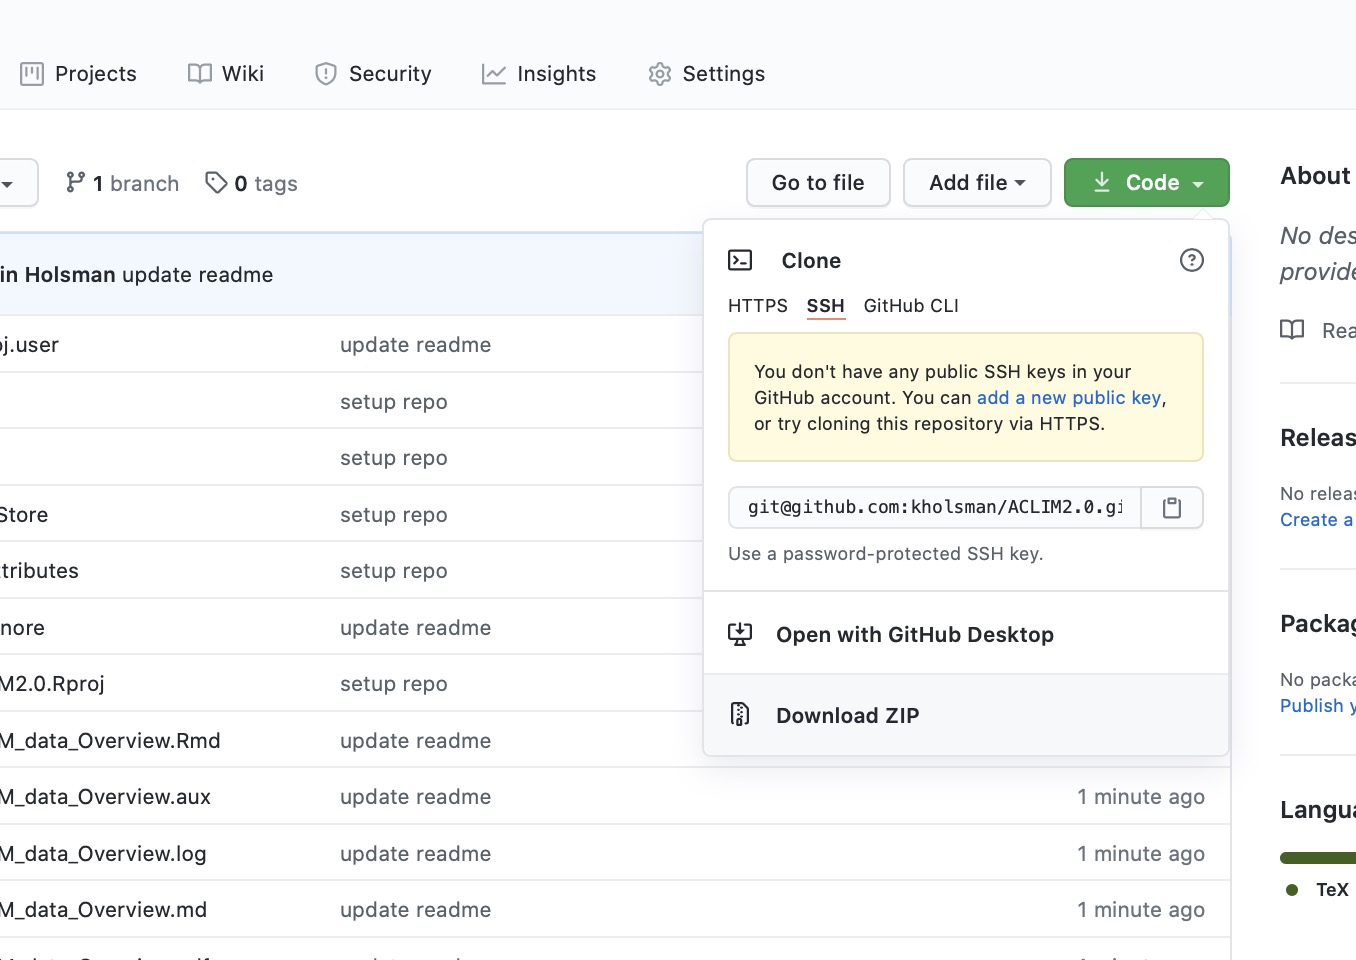
\includegraphics[width=1\textwidth,height=\textheight]{Figs/clone.jpg}

\hypertarget{get-data-step-2}{%
\section{3. Get Data (Step 2)}\label{get-data-step-2}}

The naming convention of the folders is:
\texttt{B10K-{[}ROMSNPZ\ version{]}\_{[}CMIP{]}\_{[}GCM{]}\_{[}carbon\ scenario{]}}.For
example, the CMIP5 set of indices was downscaled using the H16 (Hermann
et al.~2016) version of the ROMSNPZ. Three models were used to force
boundary conditions( MIROC, CESM, and GFDL) under 2 carbon scenarios RCP
8.5 and RCP 4.5. So to see an individual trajectory we might look in the
level3 (timeseries indices) folder under
\texttt{B10K-H16\_CMIP5\_CESM\_rcp45}, which would be the B10K version
H16 of the CMIP5 CESM model under RCP4.5.

\hypertarget{public-web-based-aclim-data-hindcasts-cmip5-projections}{%
\subsection{3.2 Public web-based ACLIM data (hindcasts \& CMIP5
projections)}\label{public-web-based-aclim-data-hindcasts-cmip5-projections}}

The naming convention of the folders is:
\texttt{B10K-{[}ROMSNPZ\ version{]}\_{[}CMIP{]}\_{[}GCM{]}\_{[}carbon\ scenario{]}}.For
example, the CMIP5 set of indices was downscaled using the H16 (Hermann
et al.~2016) version of the ROMSNPZ. Three models were used to force
boundary conditions( MIROC, CESM, and GFDL) under 2 carbon scenarios RCP
8.5 and RCP 4.5. So to see an individual trajectory we might look in the
level3 (timeseries indices) folder under
\texttt{B10K-H16\_CMIP5\_CESM\_rcp45}, which would be the B10K version
H16 of the CMIP5 CESM model under RCP4.5.

This option is available for Level3 and Level 2 CMIP5 public data, it is
not yet available for the embargoed CMIP6 data but eventually will be
used to host that as well.

The ROMSNPZ team has been working with
\href{roland.schweitzer@noaa.gov}{Roland Schweitzer} and
\href{peggy.sullivan@noaa.gov}{Peggy Sullivan} to develop the ACLIM Live
Access Server (LAS) to publicly host the published CMIP5 hindcasts and
downscaled projections. This server is in beta testing phase and can be
accessed at the following links:

\begin{itemize}
\item
  \href{https://data.pmel.noaa.gov/aclim/las/}{LAS custom ROMSNPZ data
  exploration, query, mapping, and plotting tool}
\item
  \href{https://data.pmel.noaa.gov/aclim/erddap/}{ERDAPP ACLIM data
  access tool}
\item
  \href{https://data.pmel.noaa.gov/aclim/thredds/}{THREDDS ACLIM direct
  access to Level 2 and 3 netcdf files}
\end{itemize}

\hypertarget{grab-l2-and-l3-data-from-aclim-thredds-server}{%
\subsubsection{2.2.1. Grab L2 and L3 data from ACLIM Thredds
server}\label{grab-l2-and-l3-data-from-aclim-thredds-server}}

The code below will step through downloading L3 data from the Thredds
server as well as quering the L2 (large files) on the server and saving
a subset of the data to your local
\texttt{\textasciitilde{}/ACLIM2/Data/out} folder.

First let's get the workspace set up, will we step through an example
downloading the hindcast and a single projection (CMIP5 MIROC rcp8.5)
but you can loop the code below to download the full set of CMIP5
projections.

\begin{Shaded}
\begin{Highlighting}[]
    \CommentTok{# first load packages and setup:}
\NormalTok{    tmstp  <-}\StringTok{ }\KeywordTok{format}\NormalTok{(}\KeywordTok{Sys.time}\NormalTok{(), }\StringTok{"%Y_%m_%d"}\NormalTok{)}
\NormalTok{    main   <-}\StringTok{ }\KeywordTok{getwd}\NormalTok{()    }\CommentTok{# should be your local path e.g., "~/GitHub_new/ACLIM2"}
    
    \CommentTok{# loads packages, data, and setup:}
    \KeywordTok{source}\NormalTok{(}\StringTok{"R/make.R"}\NormalTok{) }
    
    \CommentTok{# create a directory for our new indices }
    \ControlFlowTok{if}\NormalTok{(}\OperatorTok{!}\KeywordTok{dir.exists}\NormalTok{(}\StringTok{"Data/in/Newest/Rdata"}\NormalTok{)) }\KeywordTok{dir.create}\NormalTok{(}\StringTok{"Data/in/Newest/Rdata"}\NormalTok{)}
    
    \CommentTok{# specify the root URL:}
\NormalTok{    ACLIM_data_url <-}\StringTok{ "https://data.pmel.noaa.gov/aclim/thredds/"}
    
    \CommentTok{# define the threddds url}
\NormalTok{    aclim_thredds <-}\StringTok{ "https://data.pmel.noaa.gov/aclim/thredds/"}
\end{Highlighting}
\end{Shaded}

Let's take a look at the availble datasets:

\begin{Shaded}
\begin{Highlighting}[]
    \CommentTok{# preview the datasets on the server:}
\NormalTok{    url_list <-}\StringTok{ }\KeywordTok{tds_list_datasets}\NormalTok{(}\DataTypeTok{thredds_url =}\NormalTok{ ACLIM_data_url)}
    
    \CommentTok{#display the full set of datasets:}
    \KeywordTok{cat}\NormalTok{(}\KeywordTok{paste}\NormalTok{(url_list}\OperatorTok{$}\NormalTok{dataset,}\StringTok{"}\CharTok{\textbackslash{}n}\StringTok{"}\NormalTok{))}
\end{Highlighting}
\end{Shaded}

\begin{verbatim}
## Constants/ 
##  B10K-H16_CMIP5_CESM_BIO_rcp85/ 
##  B10K-H16_CMIP5_CESM_rcp45/ 
##  B10K-H16_CMIP5_CESM_rcp85/ 
##  B10K-H16_CMIP5_GFDL_BIO_rcp85/ 
##  B10K-H16_CMIP5_GFDL_rcp45/ 
##  B10K-H16_CMIP5_GFDL_rcp85/ 
##  B10K-H16_CMIP5_MIROC_rcp45/ 
##  B10K-H16_CMIP5_MIROC_rcp85/ 
##  B10K-H16_CORECFS/ 
##  B10K-K20_CORECFS/ 
##  files/
\end{verbatim}

First we will explore the Level 2 bottom temperature data on the
\href{https://data.pmel.noaa.gov/aclim/thredds/}{ACLIM Thredds server}
using the H16 hindcast and the H16 (CMIP5) projection for MIROC under
rcp8.5. The first step is to get the data urls:

\begin{Shaded}
\begin{Highlighting}[]
   \CommentTok{# define the simulation to download:}
\NormalTok{    cmip <-}\StringTok{ "CMIP5"}     \CommentTok{# Coupled Model Intercomparison Phase}
\NormalTok{    GCM  <-}\StringTok{ "MIROC"}     \CommentTok{# Global Circulation Model}
\NormalTok{    rcp  <-}\StringTok{ "rcp85"}     \CommentTok{# future carbon scenario}
\NormalTok{    mod  <-}\StringTok{ "B10K-H16"}  \CommentTok{# ROMSNPZ model}
\NormalTok{    hind <-}\StringTok{ "CORECFS"}   \CommentTok{# Hindcast}
    
    \CommentTok{# define the projection simulation:}
\NormalTok{    proj  <-}\StringTok{ }\KeywordTok{paste0}\NormalTok{(mod,}\StringTok{"_"}\NormalTok{,cmip,}\StringTok{"_"}\NormalTok{,GCM,}\StringTok{"_"}\NormalTok{,rcp)}
\NormalTok{    hind  <-}\StringTok{ }\KeywordTok{paste0}\NormalTok{(mod,}\StringTok{"_"}\NormalTok{,hind)}
    
    \CommentTok{# get the url for the projection and hindcast datasets:}
\NormalTok{    proj_url       <-}\StringTok{ }\NormalTok{url_list[url_list}\OperatorTok{$}\NormalTok{dataset }\OperatorTok{==}\StringTok{ }\KeywordTok{paste0}\NormalTok{(proj,}\StringTok{"/"}\NormalTok{),]}\OperatorTok{$}\NormalTok{path}
\NormalTok{    hind_url       <-}\StringTok{ }\NormalTok{url_list[url_list}\OperatorTok{$}\NormalTok{dataset }\OperatorTok{==}\StringTok{ }\KeywordTok{paste0}\NormalTok{(hind,}\StringTok{"/"}\NormalTok{),]}\OperatorTok{$}\NormalTok{path}
    
    \CommentTok{# preview the projection and hindcast data and data catalogs (Level 1, 2, and 3):}
\NormalTok{    proj_datasets  <-}\StringTok{ }\KeywordTok{tds_list_datasets}\NormalTok{(}\DataTypeTok{thredds_url =}\NormalTok{ proj_url)}
\NormalTok{    hind_datasets  <-}\StringTok{ }\KeywordTok{tds_list_datasets}\NormalTok{(}\DataTypeTok{thredds_url =}\NormalTok{ hind_url)}
    
    \CommentTok{# get url for the projection and hindcast Level 2 and Level 3 catalogs}
\NormalTok{    proj_l2_cat   <-}\StringTok{ }\NormalTok{proj_datasets[proj_datasets}\OperatorTok{$}\NormalTok{dataset }\OperatorTok{==}\StringTok{ "Level 2/"}\NormalTok{,]}\OperatorTok{$}\NormalTok{path}
\NormalTok{    proj_l3_cat   <-}\StringTok{ }\NormalTok{proj_datasets[proj_datasets}\OperatorTok{$}\NormalTok{dataset }\OperatorTok{==}\StringTok{ "Level 3/"}\NormalTok{,]}\OperatorTok{$}\NormalTok{path}
\NormalTok{    hind_l2_cat   <-}\StringTok{ }\NormalTok{hind_datasets[hind_datasets}\OperatorTok{$}\NormalTok{dataset }\OperatorTok{==}\StringTok{ "Level 2/"}\NormalTok{,]}\OperatorTok{$}\NormalTok{path}
\NormalTok{    hind_l3_cat   <-}\StringTok{ }\NormalTok{hind_datasets[hind_datasets}\OperatorTok{$}\NormalTok{dataset }\OperatorTok{==}\StringTok{ "Level 3/"}\NormalTok{,]}\OperatorTok{$}\NormalTok{path}
\NormalTok{    hind_l2_cat}
\end{Highlighting}
\end{Shaded}

\begin{verbatim}
## [1] "https://data.pmel.noaa.gov/aclim/thredds/B10K-H16_CORECFS/Level2.html"
\end{verbatim}

Now that we have the URLs let's take a look at the available Level2
datasets (currently temperature only, other variables available by
request to \href{kelly.kearney@noaa.gov}{Kelly Kearney}:

\begin{itemize}
\tightlist
\item
  \texttt{Bottom\ 5m} : bottom water temperature at 5 meters
\item
  \texttt{Surface\ 5m} : surface water temperature in the first 5 meters
\item
  \texttt{Integrated} : Integrated water column averages for various NPZ
  variables
\end{itemize}

\begin{Shaded}
\begin{Highlighting}[]
    \CommentTok{# preview the projection and hindcast Level 2 datasets:}
\NormalTok{    proj_l2_datasets  <-}\StringTok{ }\KeywordTok{tds_list_datasets}\NormalTok{(proj_l2_cat)}
\NormalTok{    hind_l2_datasets  <-}\StringTok{ }\KeywordTok{tds_list_datasets}\NormalTok{(hind_l2_cat)}
\NormalTok{    proj_l2_datasets}\OperatorTok{$}\NormalTok{dataset}
\end{Highlighting}
\end{Shaded}

\begin{verbatim}
## [1] "Bottom 5m"  "Surface 5m" "Integrated"
\end{verbatim}

\begin{Shaded}
\begin{Highlighting}[]
    \CommentTok{# get url for bottom temperature:}
\NormalTok{    proj_l2_BT_url   <-}\StringTok{ }\NormalTok{proj_l2_datasets[proj_l2_datasets}\OperatorTok{$}\NormalTok{dataset }\OperatorTok{==}\StringTok{ "Bottom 5m"}\NormalTok{,]}\OperatorTok{$}\NormalTok{path}
\NormalTok{    hind_l2_BT_url   <-}\StringTok{ }\NormalTok{hind_l2_datasets[hind_l2_datasets}\OperatorTok{$}\NormalTok{dataset }\OperatorTok{==}\StringTok{ "Bottom 5m"}\NormalTok{,]}\OperatorTok{$}\NormalTok{path}
\NormalTok{    proj_l2_BT_url}
\end{Highlighting}
\end{Shaded}

\begin{verbatim}
## [1] "https://data.pmel.noaa.gov/aclim/thredds/B10K-H16_CMIP5_MIROC_rcp85/Level2.html?dataset=B10K-H16_CMIP5_MIROC_rcp85_Level2_bottom5m"
\end{verbatim}

We can't preview the Level 3 datasets in the same way but they are
identical to those in the google drive and include two datasets

\begin{itemize}
\tightlist
\item
  \texttt{ACLIMsurveyrep\_B10K-H16\_CMIP5\_CESM\_BIO\_rcp85.nc} : NMFS
  Groundfish summer NBS and EBS survey replicated values for 60+
  variables
\item
  \texttt{ACLIMregion\_B10K-H16\_CMIP5\_CESM\_BIO\_rcp85.nc} : weekly
  strata averages for 60+ variables
\end{itemize}

\begin{Shaded}
\begin{Highlighting}[]
\NormalTok{    weekly_vars  }\CommentTok{# list of possible variables in the ACLIMregion_ files }
\end{Highlighting}
\end{Shaded}

\begin{verbatim}
##  [1] "region_area"          "Ben"                  "DetBen"              
##  [4] "Hsbl"                 "IceNH4"               "IceNO3"              
##  [7] "IcePhL"               "aice"                 "hice"                
## [10] "shflux"               "ssflux"               "Cop_integrated"      
## [13] "Cop_surface5m"        "EupO_integrated"      "EupO_surface5m"      
## [16] "EupS_integrated"      "EupS_surface5m"       "Iron_bottom5m"       
## [19] "Iron_integrated"      "Iron_surface5m"       "Jel_integrated"      
## [22] "Jel_surface5m"        "MZL_integrated"       "MZL_surface5m"       
## [25] "NCaO_integrated"      "NCaO_surface5m"       "NCaS_integrated"     
## [28] "NCaS_surface5m"       "NH4_bottom5m"         "NH4_integrated"      
## [31] "NH4_surface5m"        "NO3_bottom5m"         "NO3_integrated"      
## [34] "NO3_surface5m"        "PhL_integrated"       "PhL_surface5m"       
## [37] "PhS_integrated"       "PhS_surface5m"        "prod_Cop_integrated" 
## [40] "prod_EupO_integrated" "prod_EupS_integrated" "prod_Eup_integrated" 
## [43] "prod_Jel_integrated"  "prod_MZL_integrated"  "prod_NCaO_integrated"
## [46] "prod_NCaS_integrated" "prod_NCa_integrated"  "prod_PhL_integrated" 
## [49] "prod_PhS_integrated"  "salt_surface5m"       "temp_bottom5m"       
## [52] "temp_integrated"      "temp_surface5m"       "uEast_bottom5m"      
## [55] "uEast_surface5m"      "vNorth_bottom5m"      "vNorth_surface5m"    
## [58] "fracbelow0"           "fracbelow1"           "fracbelow2"
\end{verbatim}

Now let's grab some of the Level 3 and Level 2 data and store it in the
\texttt{Data/in/Newest/Rdata} folder. We'll start with Level 3 since
those files are already post-processed to be in the ACLIM indices format
and are relatively small:

\begin{Shaded}
\begin{Highlighting}[]
    \CommentTok{# define the dataset sub names:   }
\NormalTok{    weekly_flnm     <-}\StringTok{ "ACLIMregion"}
\NormalTok{    survey_rep_flnm <-}\StringTok{ "ACLIMsurveyrep"}
    
    \CommentTok{# Tinker:add additional projection scenarios here}
\NormalTok{    proj_list       <-}\StringTok{ }\NormalTok{proj    }

    
    \CommentTok{# Tinker:add additional variables to varlist}
\NormalTok{    varlist         <-}\StringTok{ }\KeywordTok{c}\NormalTok{(}
                          \StringTok{"temp_bottom5m"}\NormalTok{,    }\CommentTok{# bottom temperature,}
                          \StringTok{"NCaS_integrated"}\NormalTok{,  }\CommentTok{# Large Cop}
                          \StringTok{"Cop_integrated"}\NormalTok{,   }\CommentTok{# Small Cop}
                          \StringTok{"EupS_integrated"}\NormalTok{)  }\CommentTok{# Shelf  euphausiids}
    
              
    \CommentTok{# now grab dattat for the hindcast and projection sets:}
    \ControlFlowTok{for}\NormalTok{(m }\ControlFlowTok{in} \KeywordTok{c}\NormalTok{(hind, proj))\{}
      
\NormalTok{      TYPE <-}\StringTok{ }\DecValTok{1}
     
      \CommentTok{# create the simulation Level3 folder (and overwrite it if overwrite is set to T)}
      \ControlFlowTok{if}\NormalTok{(}\OperatorTok{!}\KeywordTok{dir.exists}\NormalTok{(}\KeywordTok{paste0}\NormalTok{(}\StringTok{"Data/in/Newest/Rdata/"}\NormalTok{,m)))}
        \KeywordTok{dir.create}\NormalTok{((}\KeywordTok{paste0}\NormalTok{(}\StringTok{"Data/in/Newest/Rdata/"}\NormalTok{,m)))}
      \ControlFlowTok{if}\NormalTok{(}\OperatorTok{!}\KeywordTok{dir.exists}\NormalTok{(}\KeywordTok{paste0}\NormalTok{(}\StringTok{"Data/in/Newest/Rdata/"}\NormalTok{,m,}\StringTok{"/Level3"}\NormalTok{)))}
        \KeywordTok{dir.create}\NormalTok{((}\KeywordTok{paste0}\NormalTok{(}\StringTok{"Data/in/Newest/Rdata/"}\NormalTok{,m,}\StringTok{"/Level3"}\NormalTok{)))}
      
      \ControlFlowTok{for}\NormalTok{(d }\ControlFlowTok{in} \KeywordTok{c}\NormalTok{(weekly_flnm,survey_rep_flnm))\{}
          
          \CommentTok{# create filename:}
\NormalTok{          tmp_fl <-}\StringTok{ }\KeywordTok{paste0}\NormalTok{(d,}\StringTok{"_"}\NormalTok{,m)}
          
          \CommentTok{# create the temporary URL}
\NormalTok{          tmpURL <-}\StringTok{ }\KeywordTok{paste0}\NormalTok{(}\KeywordTok{paste0}\NormalTok{(ACLIM_data_url,}\StringTok{"dodsC/"}\NormalTok{,m,}\StringTok{"/Level3/"}\NormalTok{),d,}\StringTok{"_"}\NormalTok{,m,}\StringTok{".nc"}\NormalTok{)}
          
          \CommentTok{# open the netcdf file remotely}
\NormalTok{          nc     <-}\StringTok{ }\KeywordTok{nc_open}\NormalTok{(tmpURL)}
          
          \CommentTok{# convert the nc files into a long data.frame for each variable}
\NormalTok{          i <-}\StringTok{ }\DecValTok{0}
          \ControlFlowTok{for}\NormalTok{(v }\ControlFlowTok{in}\NormalTok{ varlist)\{}
\NormalTok{            i <-}\StringTok{ }\NormalTok{i }\OperatorTok{+}\StringTok{ }\DecValTok{1}
\NormalTok{            tmp_var0      <-}\StringTok{ }\KeywordTok{convert2df}\NormalTok{(}\DataTypeTok{ncIN =}\NormalTok{ nc, }\DataTypeTok{type =}\NormalTok{ TYPE, }\DataTypeTok{varIN =}\NormalTok{ v)}
\NormalTok{            tmp_var0}\OperatorTok{$}\NormalTok{sim  <-}\StringTok{ }\NormalTok{tmp_fl}
            \ControlFlowTok{if}\NormalTok{(i }\OperatorTok{==}\StringTok{ }\DecValTok{1}\NormalTok{)}
\NormalTok{              tmp_var     <-}\StringTok{ }\NormalTok{tmp_var0}
            \ControlFlowTok{if}\NormalTok{(i }\OperatorTok{!=}\StringTok{ }\DecValTok{1}\NormalTok{)}
\NormalTok{              tmp_var     <-}\StringTok{ }\KeywordTok{rbind}\NormalTok{(tmp_var,tmp_var0)}
            \KeywordTok{rm}\NormalTok{(tmp_var0)}
\NormalTok{          \}}
          
          \CommentTok{# close the nc file}
          \KeywordTok{nc_close}\NormalTok{(nc)}
          
          \CommentTok{# rename the object}
          \KeywordTok{eval}\NormalTok{(}\KeywordTok{parse}\NormalTok{(}\DataTypeTok{text =}\KeywordTok{paste0}\NormalTok{(d,}\StringTok{"<-tmp_var"}\NormalTok{) ))}
          
          \CommentTok{# save the nc file in the Data/in/Newest/Rdata/ [ simulation]/Level3 folder}
\NormalTok{          tmp_path <-}\StringTok{ }\KeywordTok{file.path}\NormalTok{( }\KeywordTok{paste0}\NormalTok{(}\StringTok{"Data/in/Newest/Rdata/"}\NormalTok{,m,}\StringTok{"/Level3"}\NormalTok{),}
                                 \KeywordTok{paste0}\NormalTok{(tmp_fl,}\StringTok{".Rdata"}\NormalTok{))}
          \KeywordTok{eval}\NormalTok{(}\KeywordTok{parse}\NormalTok{(}\DataTypeTok{text =}\KeywordTok{paste0}\NormalTok{(}\StringTok{"save("}\NormalTok{,d,}\StringTok{", file=tmp_path)"}\NormalTok{)))}
\NormalTok{          TYPE     <-}\StringTok{  }\NormalTok{TYPE }\OperatorTok{+}\StringTok{ }\DecValTok{1}
\NormalTok{      \}}
\NormalTok{    \}}
\end{Highlighting}
\end{Shaded}

Now we can do the same thing and download a subset of the Level2 data
(full 10KM Lat Lon re-gridded data), here with an example of sampling on
Aug 1 of each year:

\begin{Shaded}
\begin{Highlighting}[]
    \CommentTok{# Tinker:add additional projection scenarios here}
\NormalTok{    proj_list  <-}\StringTok{ }\NormalTok{proj    }

    \CommentTok{# Currently available Level 2 variables}
\NormalTok{    ds_list     <-}\StringTok{ }\NormalTok{proj_l2_datasets}\OperatorTok{$}\NormalTok{dataset  }\CommentTok{# datasets}
\NormalTok{    sub_varlist <-}\StringTok{ }\KeywordTok{list}\NormalTok{(}
                      \StringTok{"temp"}\NormalTok{,}
                      \StringTok{"temp"}\NormalTok{,}
                      \KeywordTok{c}\NormalTok{(}\StringTok{"EupS"}\NormalTok{,}\StringTok{"Cop"}\NormalTok{,}\StringTok{"NCaS"}\NormalTok{) )  }\CommentTok{# variables to pull from each data set}
    \CommentTok{# Tinker: try subbing in other Integrated variables (3rd in the list) }
    
    \CommentTok{# Let's sample the model years as close to Aug 1 as the model timesteps run:}
\NormalTok{    tr         <-}\StringTok{ }\KeywordTok{c}\NormalTok{(}\StringTok{"-08-1 12:00:00 GMT"}\NormalTok{) }
    
    \CommentTok{# now grab dattat for the hindcast and projection sets:}
    \ControlFlowTok{for}\NormalTok{(m }\ControlFlowTok{in} \KeywordTok{c}\NormalTok{(hind, proj))\{}
      
      \CommentTok{# create the simulation Level3 folder (and overwrite it if overwrite is set to T)}
      \ControlFlowTok{if}\NormalTok{(}\OperatorTok{!}\KeywordTok{dir.exists}\NormalTok{(}\KeywordTok{paste0}\NormalTok{(}\StringTok{"Data/in/Newest/Rdata/"}\NormalTok{,m)))}
        \KeywordTok{dir.create}\NormalTok{((}\KeywordTok{paste0}\NormalTok{(}\StringTok{"Data/in/Newest/Rdata/"}\NormalTok{,m)))}
      \ControlFlowTok{if}\NormalTok{(}\OperatorTok{!}\KeywordTok{dir.exists}\NormalTok{(}\KeywordTok{paste0}\NormalTok{(}\StringTok{"Data/in/Newest/Rdata/"}\NormalTok{,m,}\StringTok{"/Level2"}\NormalTok{)))}
        \KeywordTok{dir.create}\NormalTok{((}\KeywordTok{paste0}\NormalTok{(}\StringTok{"Data/in/Newest/Rdata/"}\NormalTok{,m,}\StringTok{"/Level2"}\NormalTok{)))}
        
      \ControlFlowTok{for}\NormalTok{(d }\ControlFlowTok{in} \DecValTok{1}\OperatorTok{:}\KeywordTok{length}\NormalTok{(ds_list))\{}
            
            \CommentTok{# create filename:}
\NormalTok{            tmp_fl <-}\StringTok{ }\KeywordTok{paste0}\NormalTok{(d,}\StringTok{"_"}\NormalTok{,m)}
            
            \CommentTok{# get the url for the simulation}
\NormalTok{            m_url       <-}\StringTok{ }\NormalTok{url_list[url_list}\OperatorTok{$}\NormalTok{dataset }\OperatorTok{==}\StringTok{ }\KeywordTok{paste0}\NormalTok{(m,}\StringTok{"/"}\NormalTok{),]}\OperatorTok{$}\NormalTok{path}
            
            \CommentTok{# preview the projection and hindcast data and data catalogs (Level 1, 2, and 3):}
\NormalTok{            m_datasets  <-}\StringTok{ }\KeywordTok{tds_list_datasets}\NormalTok{(}\DataTypeTok{thredds_url =}\NormalTok{ m_url)}
            
            \CommentTok{# get Level 2 .nc file URL}
\NormalTok{            m_l2_cat       <-}\StringTok{ }\NormalTok{m_datasets[m_datasets}\OperatorTok{$}\NormalTok{dataset }\OperatorTok{==}\StringTok{ "Level 2/"}\NormalTok{,]}\OperatorTok{$}\NormalTok{path}
\NormalTok{            m_l2_datasets  <-}\StringTok{ }\KeywordTok{tds_list_datasets}\NormalTok{(m_l2_cat)}
\NormalTok{            m_l2_vT_url    <-}\StringTok{ }\NormalTok{m_l2_datasets[m_l2_datasets}\OperatorTok{$}\NormalTok{dataset }\OperatorTok{==}\StringTok{ }\NormalTok{ds_list[d],]}\OperatorTok{$}\NormalTok{path}
\NormalTok{            m_flnm         <-}\StringTok{ }\KeywordTok{strsplit}\NormalTok{(m_l2_vT_url,}\DataTypeTok{split=}\StringTok{"dataset="}\NormalTok{)[[}\DecValTok{1}\NormalTok{]][}\DecValTok{2}\NormalTok{]}
\NormalTok{            m_flnm         <-}\StringTok{ }\NormalTok{stringr}\OperatorTok{::}\KeywordTok{str_replace}\NormalTok{(m_flnm,}\StringTok{"Level2_"}\NormalTok{,}\StringTok{""}\NormalTok{)}
            \ControlFlowTok{if}\NormalTok{(ds_list[d] }\OperatorTok{==}\StringTok{"Surface 5m"}\NormalTok{) m_flnm         <-}\StringTok{ }\NormalTok{stringr}\OperatorTok{::}\KeywordTok{str_replace}\NormalTok{(m_flnm,}\StringTok{"surface_5m"}\NormalTok{,}\StringTok{"surface5m"}\NormalTok{)}
\NormalTok{            tmpURL         <-}\StringTok{ }\KeywordTok{paste0}\NormalTok{(}\KeywordTok{paste0}\NormalTok{(ACLIM_data_url,}\StringTok{"dodsC/Level2/"}\NormalTok{),m_flnm,}\StringTok{".nc"}\NormalTok{)}
            
            \CommentTok{# open the netcdf file remotely}
\NormalTok{            nc     <-}\StringTok{ }\KeywordTok{nc_open}\NormalTok{(tmpURL)}
            
            \CommentTok{# available variables:}
            \KeywordTok{names}\NormalTok{(nc}\OperatorTok{$}\NormalTok{var)}
            
\NormalTok{            time_steps  <-}\StringTok{ }\KeywordTok{as.POSIXct}\NormalTok{(}
\NormalTok{                    nc}\OperatorTok{$}\NormalTok{var[[ sub_varlist[[d]][}\DecValTok{1}\NormalTok{] ]]}\OperatorTok{$}\NormalTok{dim[[}\DecValTok{3}\NormalTok{]]}\OperatorTok{$}\NormalTok{vals, }
                    \DataTypeTok{origin =} \KeywordTok{substr}\NormalTok{(ncIN}\OperatorTok{$}\NormalTok{var[[}\StringTok{"temp"}\NormalTok{]]}\OperatorTok{$}\NormalTok{dim[[}\DecValTok{3}\NormalTok{]]}\OperatorTok{$}\NormalTok{units,}\DecValTok{15}\NormalTok{,}\DecValTok{36}\NormalTok{),}
                    \DataTypeTok{tz =} \StringTok{"GMT"}\NormalTok{) }
            
            \CommentTok{# get years in simulation}
\NormalTok{            yrs    <-}\StringTok{ }\KeywordTok{sort}\NormalTok{(}\KeywordTok{unique}\NormalTok{(}\KeywordTok{substr}\NormalTok{(time_steps,}\DecValTok{1}\NormalTok{,}\DecValTok{4}\NormalTok{)))}
\NormalTok{            tmp_tr <-}\StringTok{  }\KeywordTok{paste0}\NormalTok{(yrs,tr)}
            
            \CommentTok{# subset the lat and lon values}
\NormalTok{            lat    <-}\StringTok{ }\KeywordTok{ncvar_get}\NormalTok{(nc, }\DataTypeTok{varid =} \StringTok{"lat_rho"}\NormalTok{)}
\NormalTok{            lon    <-}\StringTok{ }\KeywordTok{ncvar_get}\NormalTok{(nc, }\DataTypeTok{varid =} \StringTok{"lon_rho"}\NormalTok{)}
            \CommentTok{#M2 <- (56.87°N, -164.06°W)}
            
            \ControlFlowTok{for}\NormalTok{(var_get }\ControlFlowTok{in}\NormalTok{ sub_varlist[[d]])\{}
               \CommentTok{# convert the nc files into a long data.frame for each variable}
\NormalTok{               tmp_var      <-}\StringTok{ }\KeywordTok{get_level2}\NormalTok{(}
                                            \DataTypeTok{ncIN =}\NormalTok{ nc, }
                                            \DataTypeTok{varIN =}\NormalTok{ var_get,     }
                                            \CommentTok{# Tinker: try extracting other vars like "NO3", or "uEast"}
                                            \DataTypeTok{xi_range  =} \DecValTok{1}\OperatorTok{:}\DecValTok{182}\NormalTok{,   }
                                            \DataTypeTok{eta_range =} \DecValTok{1}\OperatorTok{:}\DecValTok{258}\NormalTok{, }
                                            \DataTypeTok{time_range  =}\NormalTok{ tmp_tr)}
              
                \CommentTok{# rename the object}
                \KeywordTok{eval}\NormalTok{(}\KeywordTok{parse}\NormalTok{(}\DataTypeTok{text =}\KeywordTok{paste0}\NormalTok{(var_get,}\StringTok{"<-tmp_var"}\NormalTok{) ))}
              
                \CommentTok{# save the nc file in the Data/in/Newest/Rdata/ [ simulation]/Level3 folder}
\NormalTok{                tmp_path <-}\StringTok{ }\KeywordTok{file.path}\NormalTok{( }\KeywordTok{paste0}\NormalTok{(}\StringTok{"Data/in/Newest/Rdata/"}\NormalTok{,m,}\StringTok{"/Level2"}\NormalTok{),}\KeywordTok{paste0}\NormalTok{(m_flnm,}\StringTok{"_"}\NormalTok{,var_get,}\StringTok{".Rdata"}\NormalTok{))}
                \KeywordTok{eval}\NormalTok{(}\KeywordTok{parse}\NormalTok{(}\DataTypeTok{text =}\KeywordTok{paste0}\NormalTok{(}\StringTok{"save("}\NormalTok{,var_get,}\StringTok{", file=tmp_path)"}\NormalTok{)))}
                \KeywordTok{eval}\NormalTok{(}\KeywordTok{parse}\NormalTok{(}\DataTypeTok{text =}\KeywordTok{paste0}\NormalTok{(}\StringTok{"rm("}\NormalTok{,var_get,}\StringTok{")"}\NormalTok{) ))}
\NormalTok{            \}}
            \CommentTok{# close the nc file}
            \KeywordTok{nc_close}\NormalTok{(nc)}
\NormalTok{      \}}
      
\NormalTok{  \}}
\end{Highlighting}
\end{Shaded}

\begin{figure}
\centering
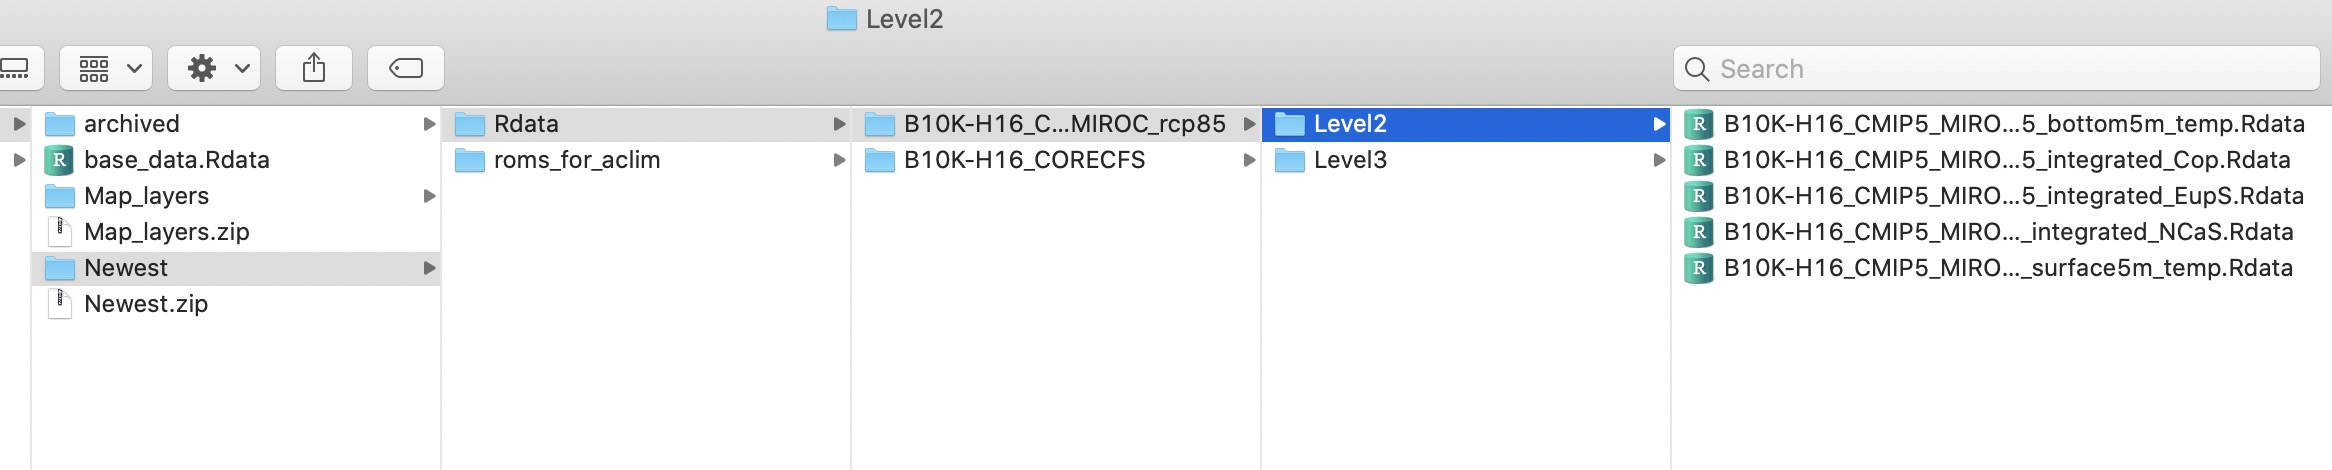
\includegraphics[width=1\textwidth,height=\textheight]{Figs/filestructure.jpg}
\caption{The final folder structure on your local drive in
\texttt{Data/in/Newest} should look something like this.}
\end{figure}

\hypertarget{aclim-members-only-access-cmip6-embargoed-l3-data}{%
\subsection{\texorpdfstring{3.2. (\emph{ACLIM members Only}) Access
CMIP6 (embargoed) L3
data}{3.2. (ACLIM members Only) Access CMIP6 (embargoed) L3 data}}\label{aclim-members-only-access-cmip6-embargoed-l3-data}}

Public CMIP5 and embargoed CMIP6 Level 3 netcdf (.nc) files are saved in
the shared ACLIM data folder (note: Level 2 files are too large for the
google drive but are available by request from
\href{kelly.kearney@noaa.gov}{Kelly Kearney}.

\textbf{IMPORTANT} Please note that while the CMIP5 set is now public
(Hermann et al.~2019; section 2.2) \textbf{the CMIP6 suite is under
embargo for QAQC and should not be shared outside of the ACLIM group}.
The ROMSNPZ team (Drs. Hermann, Cheng, Kearney, Pilcher, Adyin) are in
the process of synthesizing and publishing the CMIP6 data (goal is
spring 2021 for submission), following those publications the data will
be made accessible to the public via the PMEL data portal, as is the
case for the CMIP5 data and public hindcasts. The ROMSNPZ team has made
these runs available to ACLIM2 members in order to accelerate coupling
to biological and social and economic models, thus out of professional
courtesy please do not publish the data without permission from
\textbf{all} ROMSNPZ team members, it is strongly advised that some or
multiple ROMSNPZ team members be included as co-authors to ensure proper
application and use of the ROMSNPZ data.

For most applications you can use the ACLIM level3 post-processed
indices available on the shared ACLIM drive in the root google drive
data folder:
\href{https://drive.google.com/drive/u/0/folders/0Bx7wdZllbuF9eDJndkhCS2EwQUk}{\textbf{00\_ACLIM\_shared\textgreater02\_DATA}}.

The \texttt{Newest} folder is organized by Bering10K version, General
Circulation Model (GCM) and carbon scenario,
e.g.~\texttt{B10K-H16\_CMIP5\_CESM\_rcp45}. Within each folder the
following subfolders are:

\begin{itemize}
\tightlist
\item
  \texttt{Level1}: (Empty; not copied from Mox)
\item
  \texttt{Level2}: (Empty; not copied from Mox)
\item
  \texttt{Level3}: 2 files (\texttt{ACLIMsurveyrep\_B10K-x.nc} and
  \texttt{ACLIMregion\_B10K-x.nc} )
\end{itemize}

\begin{enumerate}
\def\labelenumi{\arabic{enumi})}
\tightlist
\item
  \texttt{ACLIMsurveyrep\_B10K-x.nc} contains summer groundfish trawl
  ``survey replicated'' indices (using mean date and lat lon)
  \emph{(Note that the resampling stations need to be removed before
  creating bottom temperature maps)}\\
\item
  \texttt{ACLIMregion\_B10K-x.nc}: contains weekly ``strata'' values
  \emph{(Note that area weighting should be used to combine values
  across multiple strata)}
\end{enumerate}

There are two folders that need to be copied into the ACLIM2 folder on
your computer under
`\texttt{\textasciitilde{}{[}YOURPATH{]}/ACLIM2/Data/in/}:

\begin{enumerate}
\def\labelenumi{\arabic{enumi})}
\item
  \href{https://drive.google.com/drive/u/0/folders/0Bx7wdZllbuF9eDJndkhCS2EwQUk}{\textbf{00\_ACLIM\_shared\textgreater02\_DATA\textgreater Newest}}.
  This folder contains a folder called \texttt{roms\_for\_aclim} with
  all the ACLIM Level3 indices for model simulations available to ACLIM
  members.
\item
  \href{https://drive.google.com/drive/u/0/folders/0Bx7wdZllbuF9eDJndkhCS2EwQUk}{\textbf{00\_ACLIM\_shared\textgreater02\_DATA\textgreater Map\_layers.zip}}.
  This file needs to be unzipped after you download it to your local
  folder. It contains (large) base maps for the code below including
  \texttt{shp\_files} and \texttt{geo\_tif} folders.
\end{enumerate}

\begin{figure}
\centering
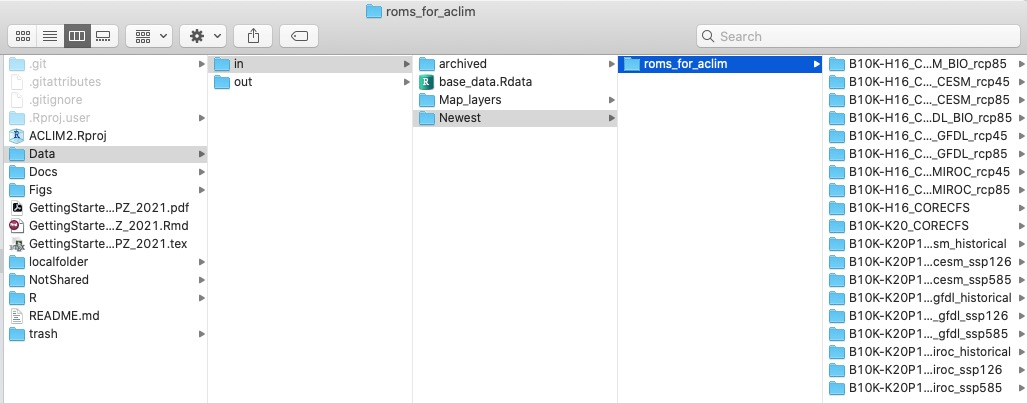
\includegraphics[width=1\textwidth,height=\textheight]{Figs/data_dir.jpg}
\caption{Your local \texttt{ACLIM2/Data} directory should look something
like this when you are done downloading the data and unzipping it.}
\end{figure}

Now let's convert these to level3 rdata files (as in section 2.2)

\begin{Shaded}
\begin{Highlighting}[]
    \CommentTok{# first load packages and setup:}
\NormalTok{    tmstp  <-}\StringTok{ }\KeywordTok{format}\NormalTok{(}\KeywordTok{Sys.time}\NormalTok{(), }\StringTok{"%Y_%m_%d"}\NormalTok{)}
\NormalTok{    main   <-}\StringTok{ }\KeywordTok{getwd}\NormalTok{()    }\CommentTok{# should be your local path e.g., "~/GitHub_new/ACLIM2"}
    
    \CommentTok{# loads packages, data, and setup:}
    \KeywordTok{source}\NormalTok{(}\StringTok{"R/make.R"}\NormalTok{) }
    
    \CommentTok{# create a directory for our new indices }
    \ControlFlowTok{if}\NormalTok{(}\OperatorTok{!}\KeywordTok{dir.exists}\NormalTok{(}\StringTok{"Data/in/Newest/Rdata"}\NormalTok{)) }\KeywordTok{dir.create}\NormalTok{(}\StringTok{"Data/in/Newest/Rdata"}\NormalTok{)}
    
    \CommentTok{# define the simulation to download:}
\NormalTok{    cmip <-}\StringTok{ "CMIP6"}     \CommentTok{# Coupled Model Intercomparison Phase}
\NormalTok{    GCM  <-}\StringTok{ "MIROC"}     \CommentTok{# Global Circulation Model}
\NormalTok{    rcp  <-}\StringTok{ "ssp585"}     \CommentTok{# future carbon scenario}
\NormalTok{    mod_h  <-}\StringTok{ "B10K-K20"}  \CommentTok{# ROMSNPZ model}
\NormalTok{    mod_p  <-}\StringTok{ "B10K-K20P19"}  \CommentTok{# ROMSNPZ model}
\NormalTok{    hind <-}\StringTok{ "CORECFS"}   \CommentTok{# Hindcast}
    
    \CommentTok{# define the projection simulation:}
\NormalTok{    proj  <-}\StringTok{ }\KeywordTok{paste0}\NormalTok{(mod_p,}\StringTok{"_"}\NormalTok{,cmip,}\StringTok{"_"}\NormalTok{,GCM,}\StringTok{"_"}\NormalTok{,rcp)}
\NormalTok{    hind  <-}\StringTok{ }\KeywordTok{paste0}\NormalTok{(mod_h,}\StringTok{"_"}\NormalTok{,hind)}
    
    \CommentTok{# define the dataset sub names:   }
\NormalTok{    weekly_flnm     <-}\StringTok{ "ACLIMregion"}
\NormalTok{    survey_rep_flnm <-}\StringTok{ "ACLIMsurveyrep"}
    
    \CommentTok{# Tinker:add additional projection scenarios here}
\NormalTok{    proj_list       <-}\StringTok{ }\NormalTok{proj    }

    
    \CommentTok{# Tinker:add additional variables to varlist}
\NormalTok{    varlist         <-}\StringTok{ }\KeywordTok{c}\NormalTok{(}
                          \StringTok{"temp_bottom5m"}\NormalTok{,    }\CommentTok{# bottom temperature,}
                          \StringTok{"NCaS_integrated"}\NormalTok{,  }\CommentTok{# Large Cop}
                          \StringTok{"Cop_integrated"}\NormalTok{,   }\CommentTok{# Small Cop}
                          \StringTok{"EupS_integrated"}\NormalTok{)  }\CommentTok{# Shelf  euphausiids}
    
              
    \CommentTok{# now grab dattat for the hindcast and projection sets:}
    \ControlFlowTok{for}\NormalTok{(m }\ControlFlowTok{in} \KeywordTok{c}\NormalTok{(hind, proj))\{}
      
\NormalTok{      TYPE <-}\StringTok{ }\DecValTok{1}
     
      \CommentTok{# create the simulation Level3 folder (and overwrite it if overwrite is set to T)}
      \ControlFlowTok{if}\NormalTok{(}\OperatorTok{!}\KeywordTok{dir.exists}\NormalTok{(}\KeywordTok{paste0}\NormalTok{(}\StringTok{"Data/in/Newest/Rdata/"}\NormalTok{,m)))}
        \KeywordTok{dir.create}\NormalTok{((}\KeywordTok{paste0}\NormalTok{(}\StringTok{"Data/in/Newest/Rdata/"}\NormalTok{,m)))}
      \ControlFlowTok{if}\NormalTok{(}\OperatorTok{!}\KeywordTok{dir.exists}\NormalTok{(}\KeywordTok{paste0}\NormalTok{(}\StringTok{"Data/in/Newest/Rdata/"}\NormalTok{,m,}\StringTok{"/Level3"}\NormalTok{)))}
        \KeywordTok{dir.create}\NormalTok{((}\KeywordTok{paste0}\NormalTok{(}\StringTok{"Data/in/Newest/Rdata/"}\NormalTok{,m,}\StringTok{"/Level3"}\NormalTok{)))}
      
      \ControlFlowTok{for}\NormalTok{(d }\ControlFlowTok{in} \KeywordTok{c}\NormalTok{(weekly_flnm,survey_rep_flnm))\{}
          
          \CommentTok{# create filename:}
\NormalTok{          tmp_fl <-}\StringTok{ }\KeywordTok{paste0}\NormalTok{(d,}\StringTok{"_"}\NormalTok{,m)}
          
          \CommentTok{# create the temporary URL}
\NormalTok{          tmppath <-}\StringTok{ }\KeywordTok{paste0}\NormalTok{(}\KeywordTok{paste0}\NormalTok{(}\StringTok{"Data/in/Newest/roms_for_aclim/"}\NormalTok{,m,}\StringTok{"/Level3/"}\NormalTok{),d,}\StringTok{"_"}\NormalTok{,m,}\StringTok{".nc"}\NormalTok{)}
          
          \CommentTok{# open the netcdf file remotely}
\NormalTok{          nc     <-}\StringTok{ }\KeywordTok{nc_open}\NormalTok{(tmppath)}
          
          \CommentTok{# convert the nc files into a long data.frame for each variable}
\NormalTok{          i <-}\StringTok{ }\DecValTok{0}
          \ControlFlowTok{for}\NormalTok{(v }\ControlFlowTok{in}\NormalTok{ varlist)\{}
\NormalTok{            i <-}\StringTok{ }\NormalTok{i }\OperatorTok{+}\StringTok{ }\DecValTok{1}
\NormalTok{            tmp_var0      <-}\StringTok{ }\KeywordTok{convert2df}\NormalTok{(}\DataTypeTok{ncIN =}\NormalTok{ nc, }\DataTypeTok{type =}\NormalTok{ TYPE, }\DataTypeTok{varIN =}\NormalTok{ v)}
\NormalTok{            tmp_var0}\OperatorTok{$}\NormalTok{sim  <-}\StringTok{ }\NormalTok{tmp_fl}
            \ControlFlowTok{if}\NormalTok{(i }\OperatorTok{==}\StringTok{ }\DecValTok{1}\NormalTok{)}
\NormalTok{              tmp_var     <-}\StringTok{ }\NormalTok{tmp_var0}
            \ControlFlowTok{if}\NormalTok{(i }\OperatorTok{!=}\StringTok{ }\DecValTok{1}\NormalTok{)}
\NormalTok{              tmp_var     <-}\StringTok{ }\KeywordTok{rbind}\NormalTok{(tmp_var,tmp_var0)}
            \KeywordTok{rm}\NormalTok{(tmp_var0)}
\NormalTok{          \}}
          
          \CommentTok{# close the nc file}
          \KeywordTok{nc_close}\NormalTok{(nc)}
          
          \CommentTok{# rename the object}
          \KeywordTok{eval}\NormalTok{(}\KeywordTok{parse}\NormalTok{(}\DataTypeTok{text =}\KeywordTok{paste0}\NormalTok{(d,}\StringTok{"<-tmp_var"}\NormalTok{) ))}
          
          \CommentTok{# save the nc file in the Data/in/Newest/Rdata/ [ simulation]/Level3 folder}
\NormalTok{          tmp_path <-}\StringTok{ }\KeywordTok{file.path}\NormalTok{( }\KeywordTok{paste0}\NormalTok{(}\StringTok{"Data/in/Newest/Rdata/"}\NormalTok{,m,}\StringTok{"/Level3"}\NormalTok{),}
                                 \KeywordTok{paste0}\NormalTok{(tmp_fl,}\StringTok{".Rdata"}\NormalTok{))}
          \KeywordTok{eval}\NormalTok{(}\KeywordTok{parse}\NormalTok{(}\DataTypeTok{text =}\KeywordTok{paste0}\NormalTok{(}\StringTok{"save("}\NormalTok{,d,}\StringTok{", file=tmp_path)"}\NormalTok{)))}
\NormalTok{          TYPE     <-}\StringTok{  }\NormalTok{TYPE }\OperatorTok{+}\StringTok{ }\DecValTok{1}
\NormalTok{      \}}
\NormalTok{    \}}
\end{Highlighting}
\end{Shaded}

\hypertarget{derive-indices-plot-data}{%
\section{4. Derive indices \& plot
data}\label{derive-indices-plot-data}}

\hypertarget{level-3-indices}{%
\subsection{4.1 Level 3 indices:}\label{level-3-indices}}

Level 3 indices can be used to generate seasonal, monthly, and annual
indices (like those reported in
\href{https://www.frontiersin.org/articles/10.3389/fmars.2020.00124/full}{Reum
et al.~2020)},
\href{http://dx.doi.org/10.1038/s41467-020-18300-3}{Holsman et
al.~2020)}. In section 3 below we explore these indices in more detail
using R, including using (2) above to generate weekly, monthly, and
seasonal indices (e.g.~Fall Zooplankton) for use in biological models.
In section 3 below we explore these indices in more detail using R,
including using (2) above to generate weekly, monthly, and seasonal
indices (e.g.~Fall Zooplankton) for use in biological models.

Please be sure to coordinate with ROMSNPZ modeling team members to
ensure data is applied appropriately. If you need access to the raw
ROMSNPZ files (netcdf, non-regridded large files located on MOX). Please
contact \href{albert.j.hermann@noaa.gov}{\textbf{Al Hermann}} or
\href{kelly.kearney@noaa.gov}{\textbf{Kelly Kearney}}.

The following examples show how to analyze and plot the ACLIM indices
from their stored netcdf (.nc) format in the Data folder of the ACLIM
shared google drive. Please note that while the CMIP5 set is now public
(Hermann et al.~2019) \textbf{the CMIP6 suite is under embargo for QAQC
and should not be shared outside of the ACLIM group}. Al, Wei, Kelly,
Darren, and Kerim are in the process of synthesizing and publishing the
CMIP6 data (goal is spring 2021 for submission), following those
publications the data will be made accessible to the public via the PMEL
data portal, as is the case for the CMIP5 data and public hindcasts. It
is strongly recommended that you include at least one (ideally multiple)
authors from the ROMSNPZ team as co-author on your paper if you are
linking to this data, this is especially the case for the CMIP6 data.
There are multiple spatial and temporal caveats that are best described
in discussions with the authors of these data and inclusion as
co-authors will facilitate appropriate application and interpretation of
the ROMSNPZ data.

\hypertarget{explore-level-3-data-catalog}{%
\subsubsection{4.1.1 Explore Level 3 data
catalog}\label{explore-level-3-data-catalog}}

Once the base files and setup are loaded you can explore the index
types. Recall that in each scenario folder there are two indices saved
within the \texttt{Level3} subfolders:

\begin{enumerate}
\def\labelenumi{\arabic{enumi})}
\tightlist
\item
  \texttt{ACLIMsurveyrep\_B10K-x.nc} contains summer groundfish trawl
  ``survey replicated'' indices (using mean date and lat lon)
  \emph{(Note that the resampling stations need to be removed before
  creating bottom temperature maps)}\\
\item
  \texttt{ACLIMregion\_B10K-x.nc}: contains weekly ``strata'' values
  \emph{(Note that area weighting should be used to combine values
  across multiple strata)}
\end{enumerate}

First run the below set of code to set up the workspace:

\begin{Shaded}
\begin{Highlighting}[]
\NormalTok{    tmstp  <-}\StringTok{ }\KeywordTok{format}\NormalTok{(}\KeywordTok{Sys.time}\NormalTok{(), }\StringTok{"%Y_%m_%d"}\NormalTok{)}
\NormalTok{    main   <-}\StringTok{ }\KeywordTok{getwd}\NormalTok{()  }\CommentTok{#"~/GitHub_new/ACLIM2"}
    
    \CommentTok{# loads packages, data, setup, etc.}
    \KeywordTok{source}\NormalTok{(}\StringTok{"R/make.R"}\NormalTok{)}
    
    \CommentTok{# list of the scenario x GCM downscaled ACLIM indices}
    \ControlFlowTok{for}\NormalTok{(k }\ControlFlowTok{in}\NormalTok{ aclim)}
     \KeywordTok{cat}\NormalTok{(}\KeywordTok{paste}\NormalTok{(k,}\StringTok{"}\CharTok{\textbackslash{}n}\StringTok{"}\NormalTok{))}
    
\NormalTok{    embargoed }\CommentTok{# not yet public or published}
\NormalTok{    public    }\CommentTok{# published runs (CMIP5)}
    
    \CommentTok{# get some info about a scenario:}
  
\NormalTok{    all_info1 <-}\StringTok{ }\KeywordTok{info}\NormalTok{(}\DataTypeTok{model_list=}\NormalTok{aclim,}\DataTypeTok{type=}\DecValTok{1}\NormalTok{)}
\NormalTok{    all_info2 <-}\StringTok{ }\KeywordTok{info}\NormalTok{(}\DataTypeTok{model_list=}\NormalTok{aclim,}\DataTypeTok{type=}\DecValTok{2}\NormalTok{)}
\NormalTok{    all_info1}
\NormalTok{    all_info2}
   
    \CommentTok{# variables in each of the two files:}
\NormalTok{    srvy_vars}
\NormalTok{    weekly_vars}
  
    \CommentTok{#summary tables for variables}
\NormalTok{    srvy_var_def}
\NormalTok{    weekly_var_def}
    
    \CommentTok{# explore stations in the survey replicated data:}
    \KeywordTok{head}\NormalTok{(station_info)}
\end{Highlighting}
\end{Shaded}

\hypertarget{spatial-indices-survey-replicated}{%
\subsubsection{4.1.2 Spatial indices (survey
replicated)}\label{spatial-indices-survey-replicated}}

Let's start b exploring the survey replicated values for each variable.
Steps 2 and 3 generated the Rdata files that are stored in the
\texttt{ACLIMsurveyrep\_B10K-{[}version\_CMIPx\_GCM\_RCP{]}.Rdata} in
each corresponding simulation folder.

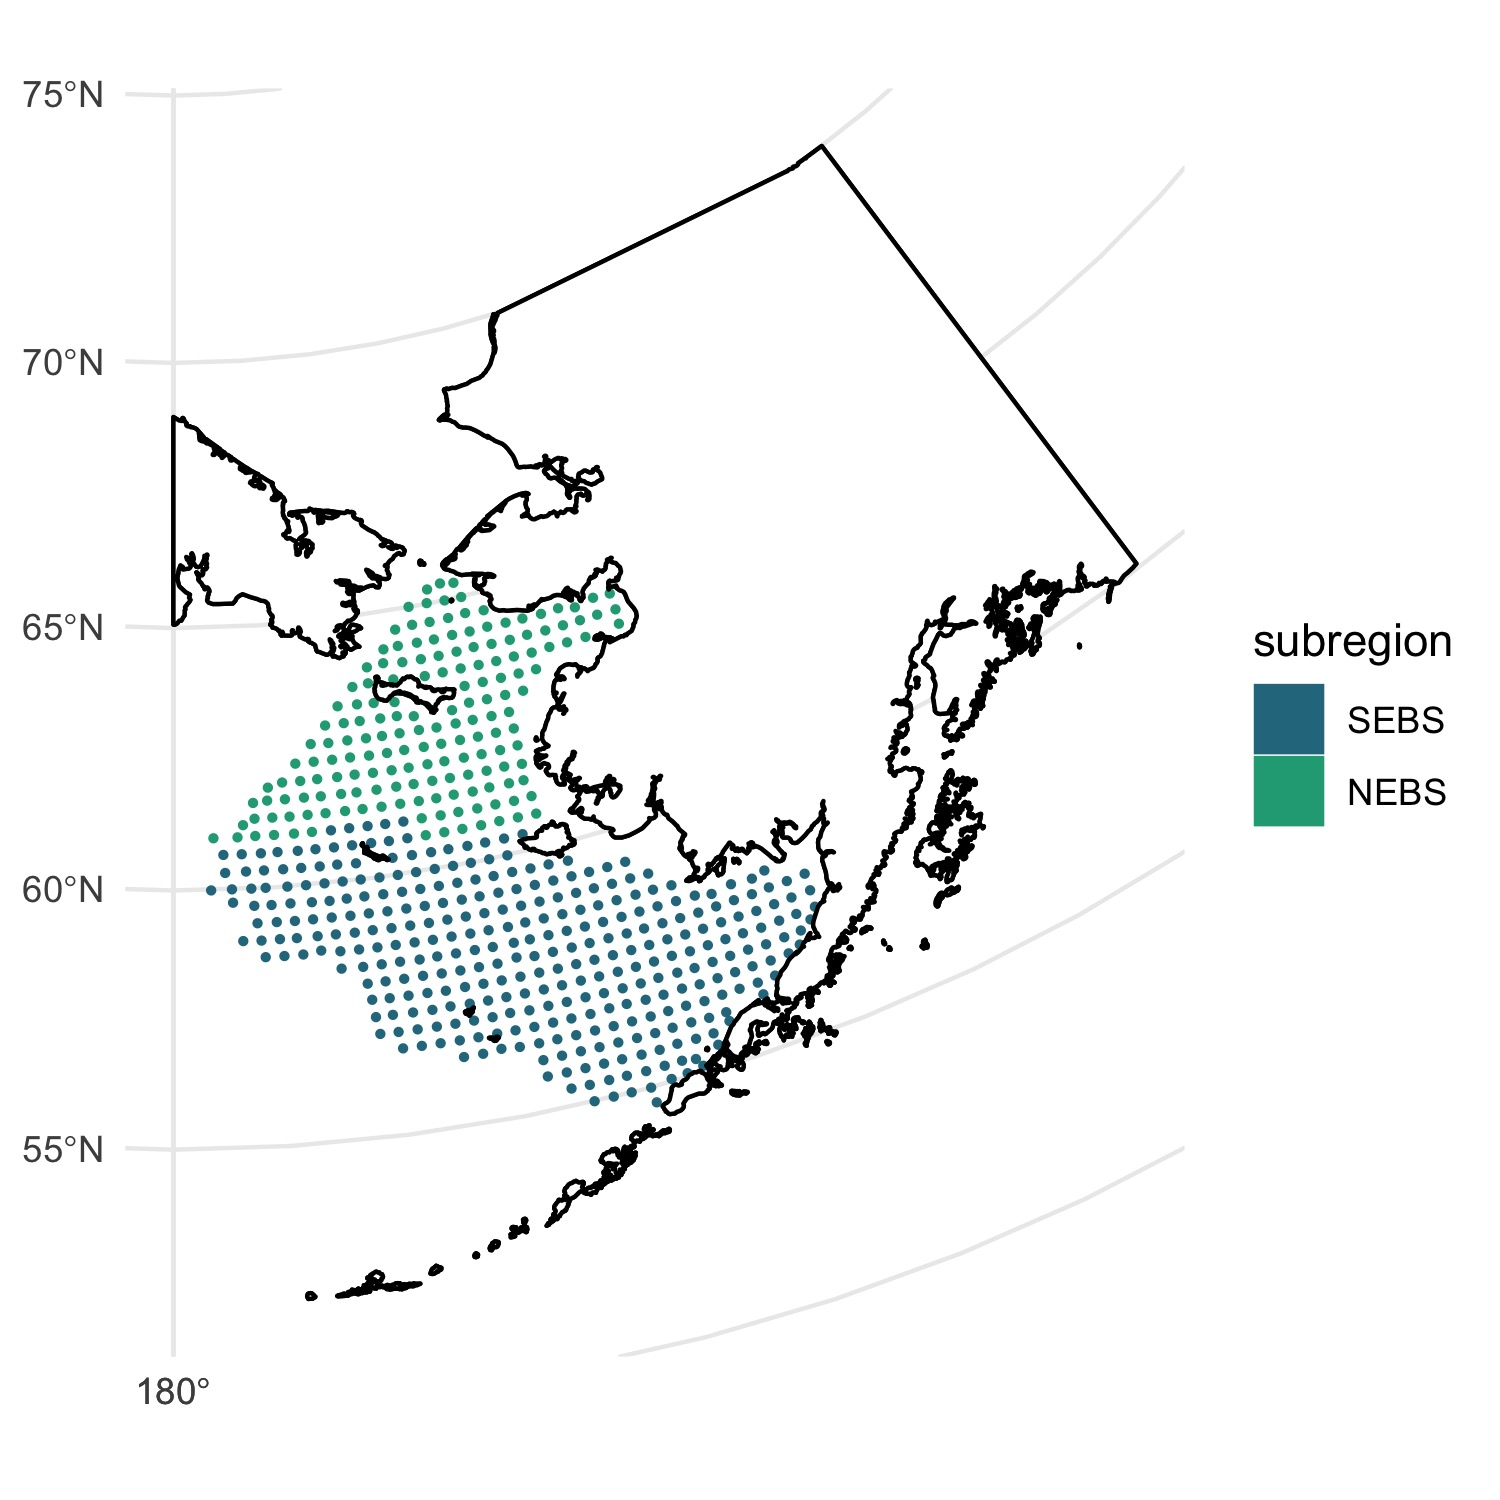
\includegraphics[width=0.5\textwidth,height=\textheight]{Figs/stations_NS.jpg}
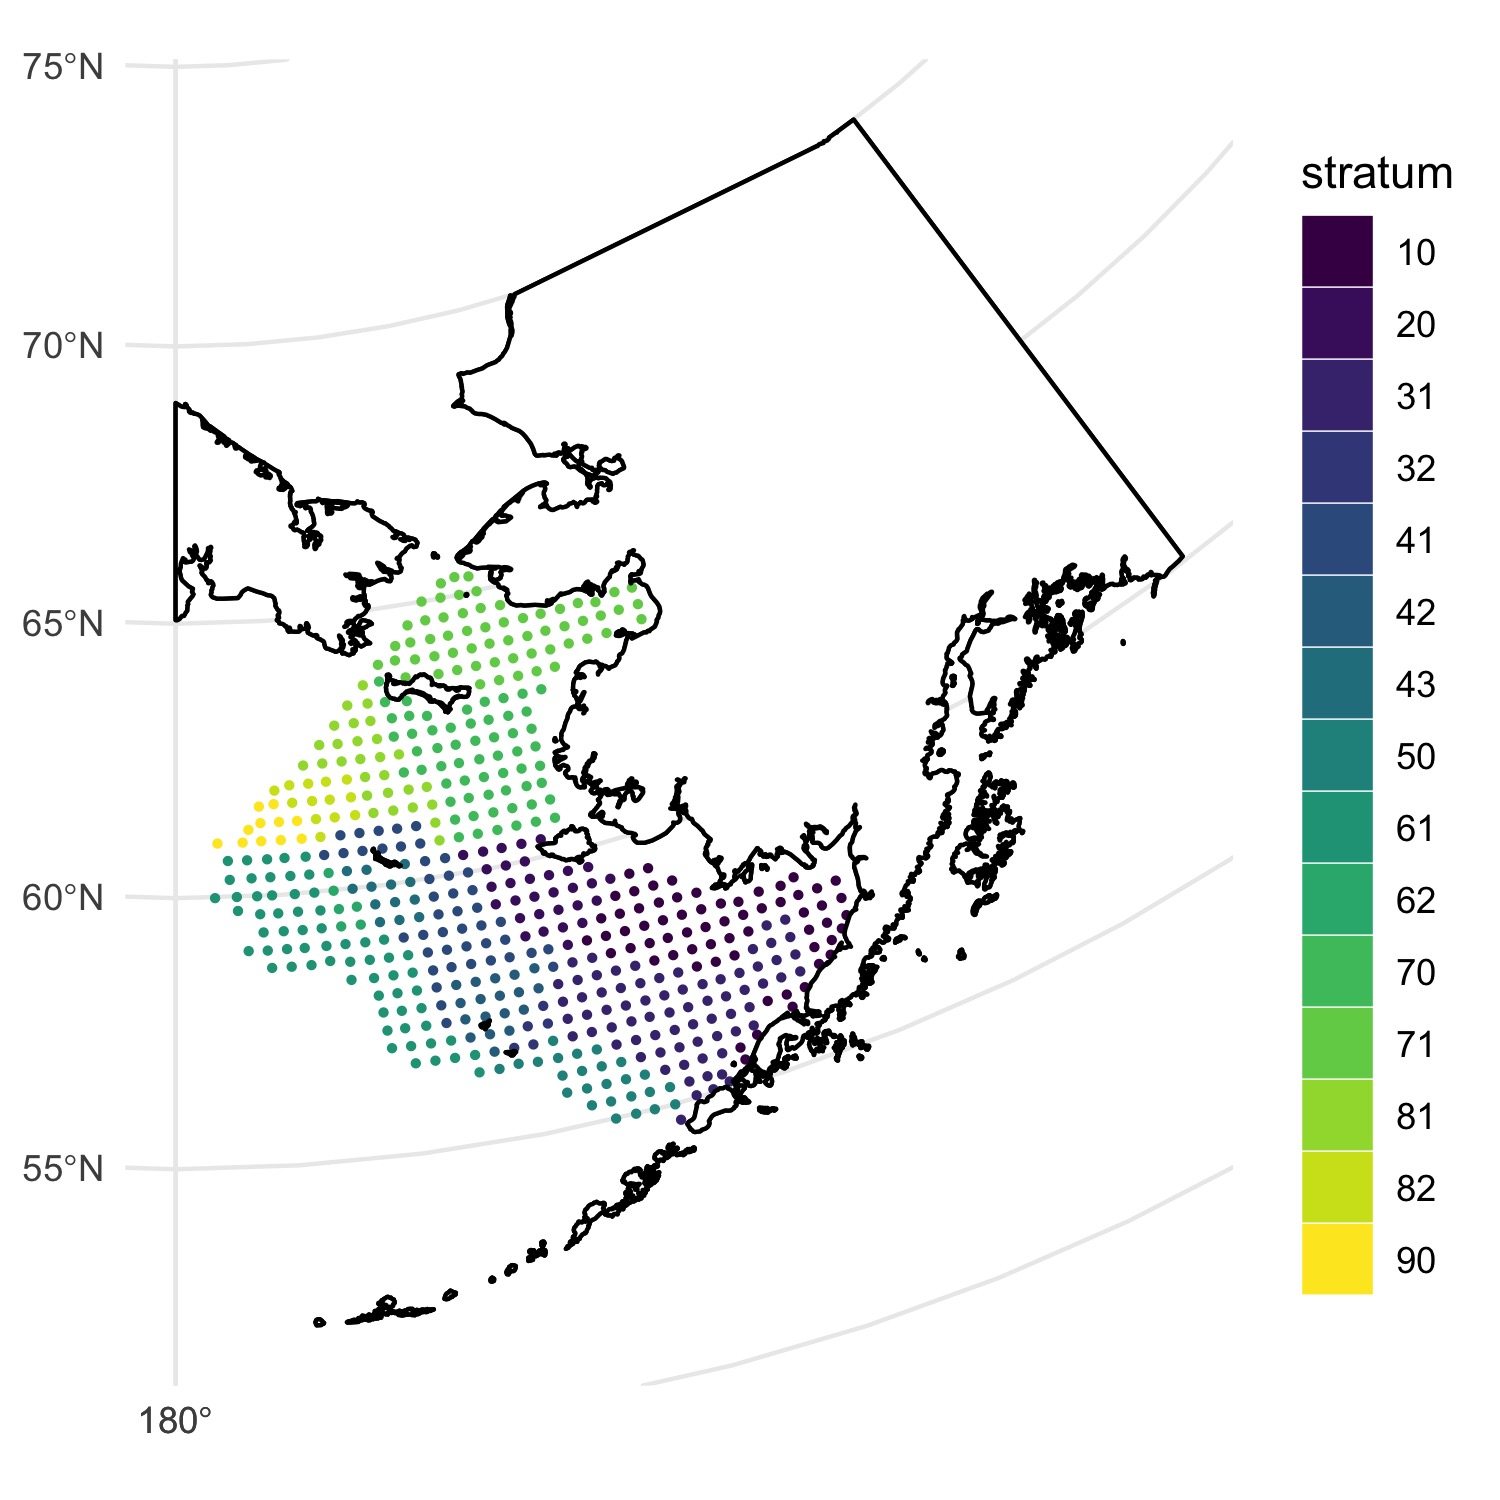
\includegraphics[width=0.5\textwidth,height=\textheight]{Figs/stations.jpg}

The code segment below will recreate the above figures.

\begin{Shaded}
\begin{Highlighting}[]
   \CommentTok{# first convert the station_info object into a shapefile for mapping:}
\NormalTok{   station_sf         <-}\StringTok{ }\KeywordTok{convert2shp}\NormalTok{(station_info)}
\NormalTok{   station_sf}\OperatorTok{$}\NormalTok{stratum <-}\StringTok{ }\KeywordTok{factor}\NormalTok{(station_sf}\OperatorTok{$}\NormalTok{stratum)}
   
   \CommentTok{# plot the stations:}
\NormalTok{   p <-}\StringTok{ }\KeywordTok{plot_stations_basemap}\NormalTok{(}\DataTypeTok{sfIN =}\NormalTok{ station_sf,}\DataTypeTok{fillIN =} \StringTok{"subregion"}\NormalTok{,}\DataTypeTok{colorIN =} \StringTok{"subregion"}\NormalTok{) }\OperatorTok{+}\StringTok{ }
\StringTok{     }\KeywordTok{scale_color_viridis_d}\NormalTok{(}\DataTypeTok{begin =} \FloatTok{.4}\NormalTok{,}\DataTypeTok{end=}\NormalTok{.}\DecValTok{6}\NormalTok{) }\OperatorTok{+}
\StringTok{     }\KeywordTok{scale_fill_viridis_d}\NormalTok{(}\DataTypeTok{begin =} \FloatTok{.4}\NormalTok{,}\DataTypeTok{end=}\NormalTok{.}\DecValTok{6}\NormalTok{)}
  
   \ControlFlowTok{if}\NormalTok{(update.figs)\{}
\NormalTok{     p}
     \KeywordTok{ggsave}\NormalTok{(}\DataTypeTok{file=}\StringTok{"Figs/stations_NS.jpg"}\NormalTok{,}\DataTypeTok{width=}\DecValTok{5}\NormalTok{,}\DataTypeTok{height=}\DecValTok{5}\NormalTok{)\}}

\NormalTok{   p2 <-}\StringTok{ }\KeywordTok{plot_stations_basemap}\NormalTok{(}\DataTypeTok{sfIN =}\NormalTok{ station_sf,}\DataTypeTok{fillIN =} \StringTok{"stratum"}\NormalTok{,}\DataTypeTok{colorIN =} \StringTok{"stratum"}\NormalTok{) }\OperatorTok{+}\StringTok{ }
\StringTok{     }\KeywordTok{scale_color_viridis_d}\NormalTok{() }\OperatorTok{+}
\StringTok{     }\KeywordTok{scale_fill_viridis_d}\NormalTok{()}
   
   \ControlFlowTok{if}\NormalTok{(update.figs)\{}
\NormalTok{     p2}
   \KeywordTok{ggsave}\NormalTok{(}\DataTypeTok{file=}\StringTok{"Figs/stations.jpg"}\NormalTok{,}\DataTypeTok{width=}\DecValTok{5}\NormalTok{,}\DataTypeTok{height=}\DecValTok{5}\NormalTok{)\}}
\end{Highlighting}
\end{Shaded}

Now let's explore the survey replicated data in more detail and use it
to create a cold pool index for each simulation and hindcast scenario x
model x CMIP combination.

\begin{Shaded}
\begin{Highlighting}[]
    \CommentTok{# now create plots of average BT during four time periods}
\NormalTok{    time_seg   <-}\StringTok{ }\KeywordTok{list}\NormalTok{(}\StringTok{'2010-2020'}\NormalTok{ =}\StringTok{ }\KeywordTok{c}\NormalTok{(}\DecValTok{2010}\OperatorTok{:}\DecValTok{2020}\NormalTok{),}
                        \StringTok{'2021-2040'}\NormalTok{ =}\StringTok{ }\KeywordTok{c}\NormalTok{(}\DecValTok{2021}\OperatorTok{:}\DecValTok{2040}\NormalTok{),}
                        \StringTok{'2041-2060'}\NormalTok{ =}\StringTok{ }\KeywordTok{c}\NormalTok{(}\DecValTok{2041}\OperatorTok{:}\DecValTok{2060}\NormalTok{),}
                        \StringTok{'2061-2080'}\NormalTok{ =}\StringTok{ }\KeywordTok{c}\NormalTok{(}\DecValTok{2061}\OperatorTok{:}\DecValTok{2080}\NormalTok{),}
                        \StringTok{'2081-2099'}\NormalTok{ =}\StringTok{ }\KeywordTok{c}\NormalTok{(}\DecValTok{2081}\OperatorTok{:}\DecValTok{2099}\NormalTok{))}
  
    \CommentTok{# View an individual variable (e.g., Bottom Temp)}
    \CommentTok{# -------------------------------------------------------}
\NormalTok{    srvy_vars}
\NormalTok{    aclim}
\NormalTok{    sim <-}\StringTok{"B10K-K20P19_CMIP6_miroc_ssp585"} 
\NormalTok{    Rdata_path <-}\StringTok{ "/Users/kholsman/GitHub_new/ACLIM2/Data/in/Newest/Rdata"}
    
    \CommentTok{# open a "region" or strata specific nc file}
\NormalTok{    fl      <-}\StringTok{ }\KeywordTok{file.path}\NormalTok{(sim,}\KeywordTok{paste0}\NormalTok{(srvy_txt,sim,}\StringTok{".Rdata"}\NormalTok{))}
    
    \CommentTok{# load object 'ACLIMsurveyrep'}
    \KeywordTok{load}\NormalTok{(}\KeywordTok{file.path}\NormalTok{(Rdata_path,fl))   }
    
    \CommentTok{# Collate mean values across timeperiods and simulations}
    \CommentTok{# -------------------------------------------------------}
\NormalTok{    m_set      <-}\StringTok{ }\KeywordTok{c}\NormalTok{(}\DecValTok{18}\NormalTok{,}\DecValTok{19}\NormalTok{)}
\NormalTok{    ms         <-}\StringTok{ }\NormalTok{aclim[m_set]}
\NormalTok{    ms         <-}\StringTok{ }\KeywordTok{c}\NormalTok{(}\StringTok{"B10K-H16_CMIP5_miroc_rcp85"}\NormalTok{,}\StringTok{"B10K-K20P19_CMIP6_miroc_ssp585"}\NormalTok{)}
    
    \CommentTok{# get the mean values for the time blocks}
\NormalTok{    mn_var_all <-}\StringTok{ }\KeywordTok{get_mn_rd}\NormalTok{(}\DataTypeTok{modset =}\NormalTok{ ms ,}\DataTypeTok{varUSE=}\StringTok{"temp_bottom5m"}\NormalTok{)}
    
    \CommentTok{# convert results to a shapefile}
\NormalTok{    mn_var_sf  <-}\StringTok{ }\KeywordTok{convert2shp}\NormalTok{(mn_var_all}\OperatorTok\KeywordTok{filter}\NormalTok{(}\OperatorTok{!}\KeywordTok{is.na}\NormalTok{(mnval)))}
\NormalTok{    lab_t       <-}\StringTok{ }\NormalTok{ms[}\DecValTok{1}\NormalTok{]}\OperatorTok\NormalTok{stringr}\OperatorTok{::}\KeywordTok{str_remove}\NormalTok{(}\StringTok{"([^-])"}\NormalTok{)}
    
\NormalTok{    p3         <-}\StringTok{ }\KeywordTok{plot_stations_basemap}\NormalTok{(}\DataTypeTok{sfIN =}\NormalTok{ mn_var_sf,}
                                \DataTypeTok{fillIN =} \StringTok{"mnval"}\NormalTok{,}
                                \DataTypeTok{colorIN =} \StringTok{"mnval"}\NormalTok{,}
                                \DataTypeTok{sizeIN=}\NormalTok{.}\DecValTok{3}\NormalTok{) }\OperatorTok{+}
\StringTok{      }\KeywordTok{facet_grid}\NormalTok{(simulation}\OperatorTok{~}\NormalTok{time_period)}\OperatorTok{+}
\StringTok{      }\KeywordTok{scale_color_viridis_c}\NormalTok{()}\OperatorTok{+}
\StringTok{      }\KeywordTok{scale_fill_viridis_c}\NormalTok{()}\OperatorTok{+}
\StringTok{      }\KeywordTok{guides}\NormalTok{(}
        \DataTypeTok{color =}  \KeywordTok{guide_legend}\NormalTok{(}\DataTypeTok{title=}\StringTok{"Bottom T (degC)"}\NormalTok{),}
        \DataTypeTok{fill  =}  \KeywordTok{guide_legend}\NormalTok{(}\DataTypeTok{title=}\StringTok{"Bottom T (degC)"}\NormalTok{)) }\OperatorTok{+}
\StringTok{      }\KeywordTok{ggtitle}\NormalTok{(lab_t)}
   
    \CommentTok{# This is slow but it works (repeat dev.new() twice if in Rstudio)...}
    \KeywordTok{dev.new}\NormalTok{()}
\NormalTok{    p3}
    
    \ControlFlowTok{if}\NormalTok{(update.figs)  }\KeywordTok{ggsave}\NormalTok{(}\DataTypeTok{file=}\StringTok{"Figs/mn_BT.jpg"}\NormalTok{,}\DataTypeTok{width=}\DecValTok{8}\NormalTok{,}\DataTypeTok{height=}\DecValTok{5}\NormalTok{)}
  
    \KeywordTok{graphics.off}\NormalTok{()}
\end{Highlighting}
\end{Shaded}

\begin{figure}
\centering
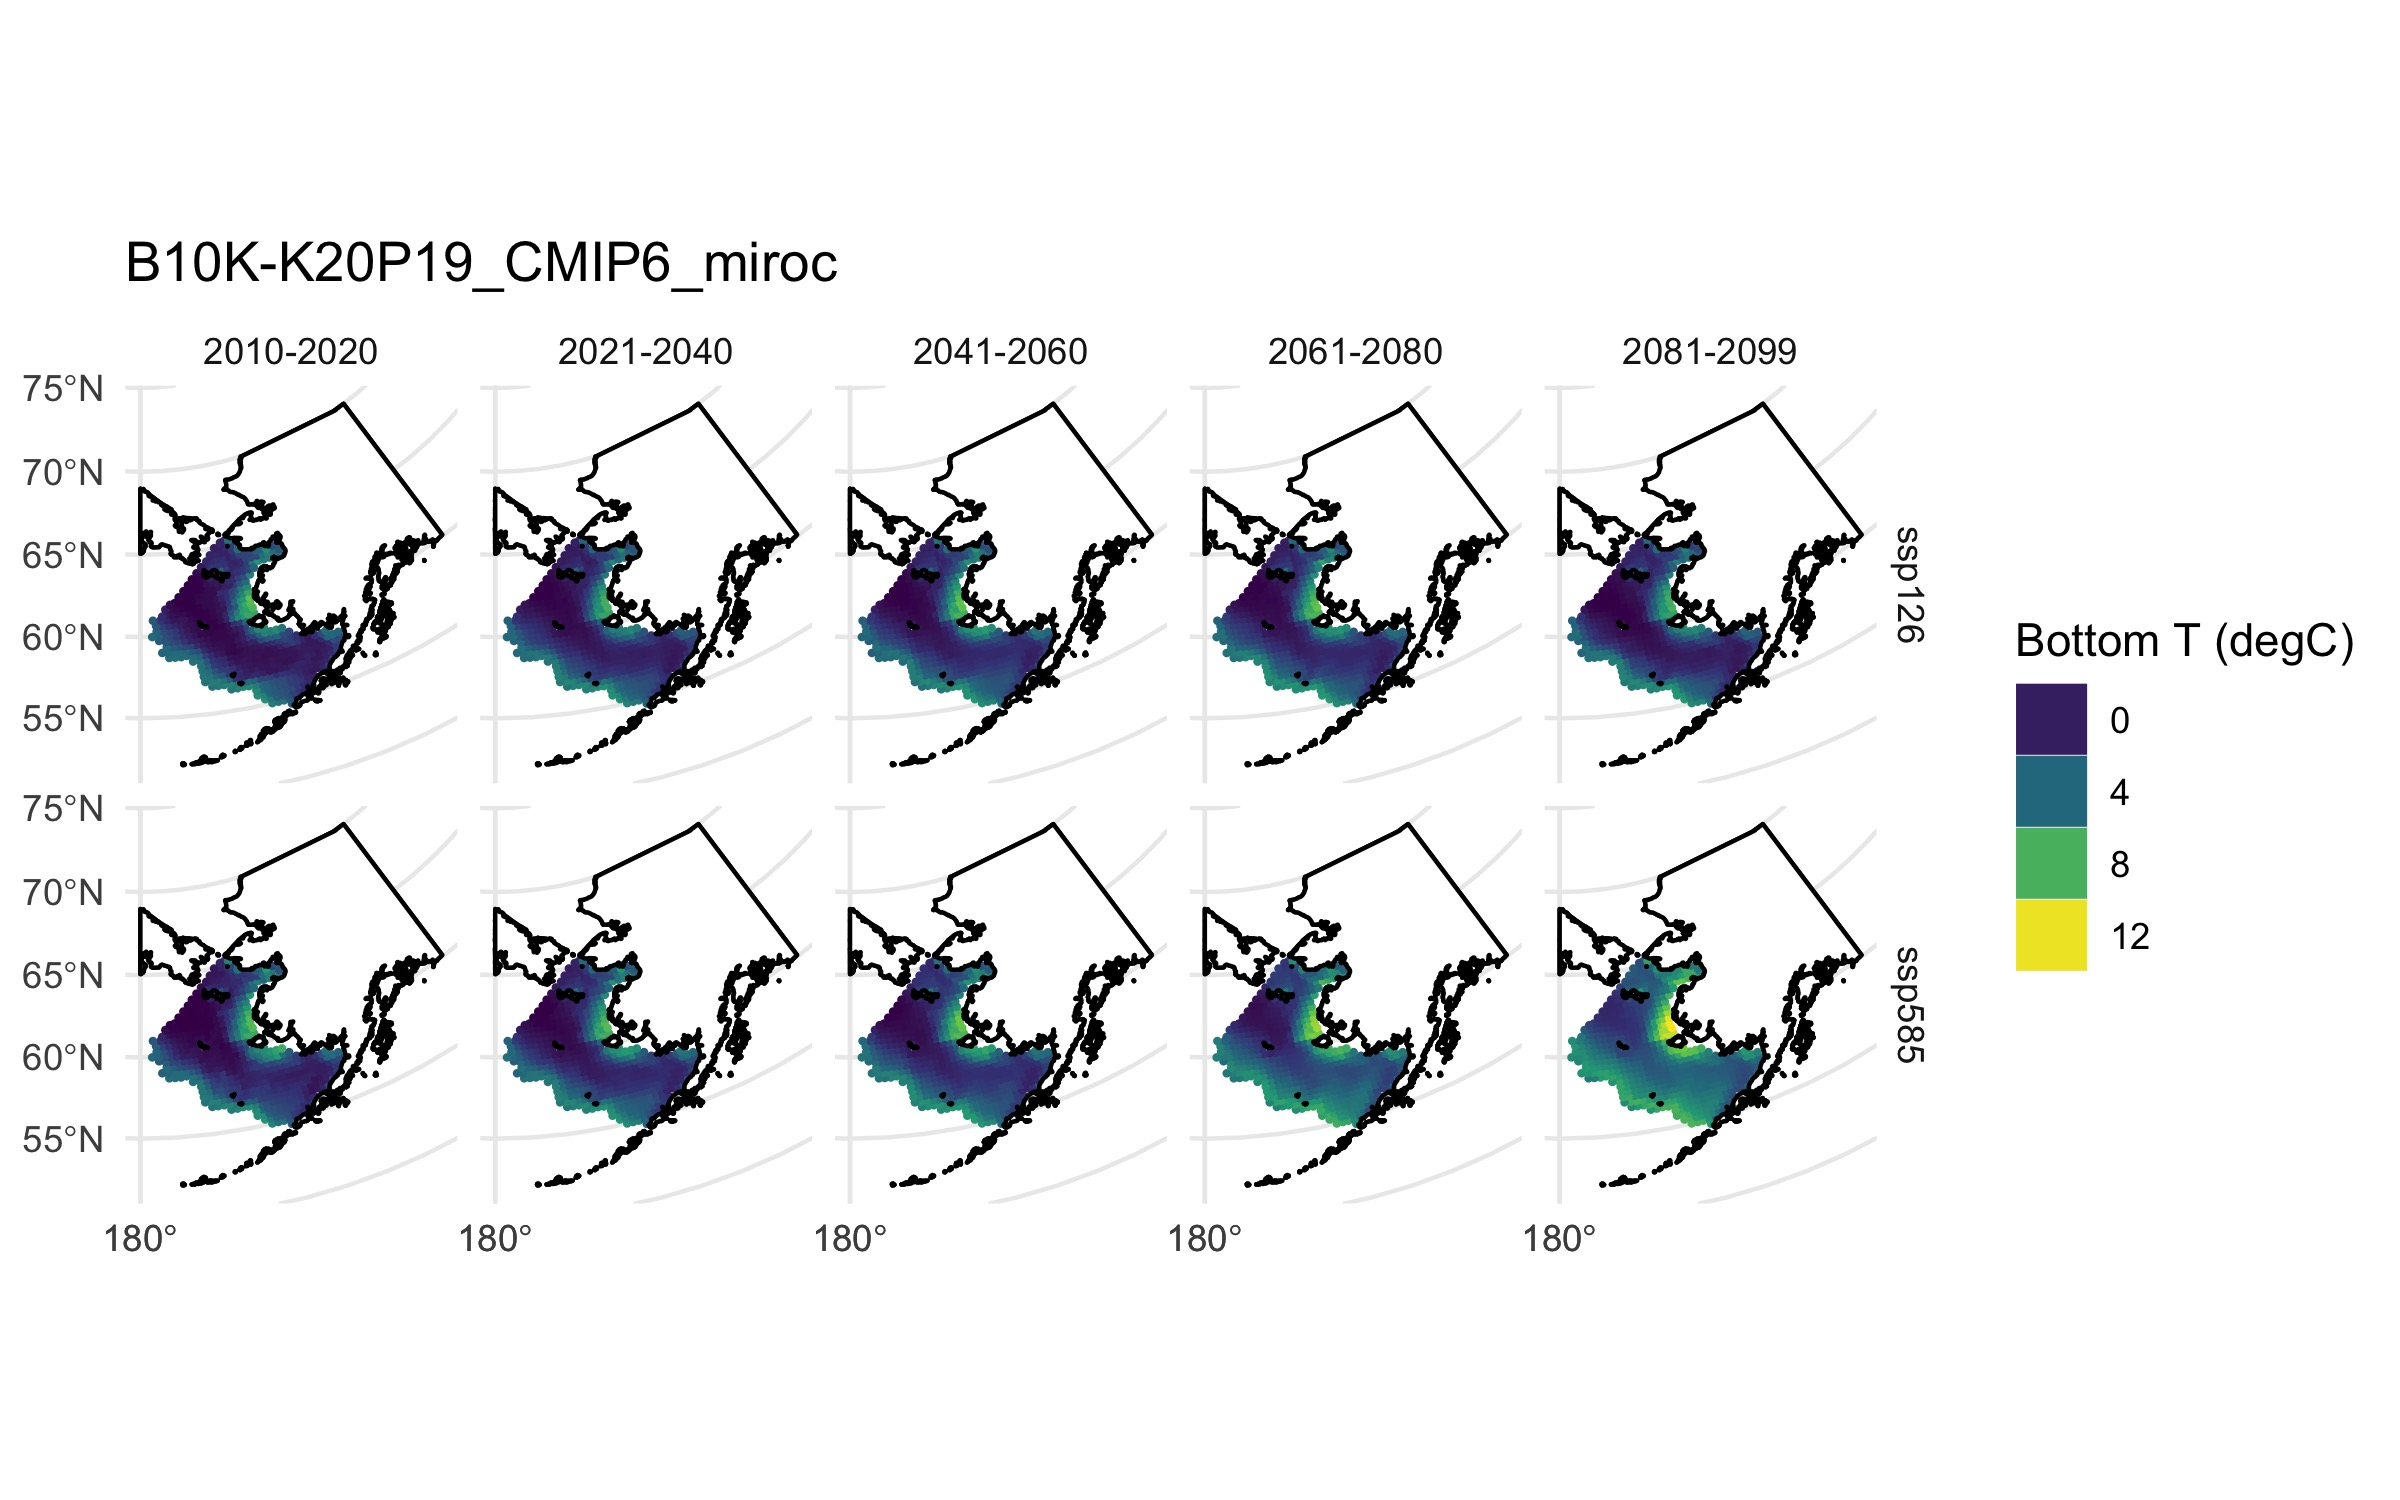
\includegraphics{Figs/mn_BT.jpg}
\caption{Bottom temperature projections under differing SSP126 (top row)
and SSP585 (bottom row)}
\end{figure}

\hypertarget{temporal-indices-weekly-strata-averages}{%
\subsubsection{4.1.3 Temporal indices (Weekly strata
averages)}\label{temporal-indices-weekly-strata-averages}}

The next set of indices to will explore are the weekly strata-specific
values for each variable.These are stored in the
\texttt{ACLIMregion\_B10K-{[}version\_CMIPx\_GCM\_RCP{]}.nc} in each
scenario folder.

\begin{Shaded}
\begin{Highlighting}[]
    \CommentTok{# list of the scenario x GCM downscaled ACLIM indices}
    \ControlFlowTok{for}\NormalTok{(k }\ControlFlowTok{in}\NormalTok{ aclim)}
      \KeywordTok{cat}\NormalTok{(}\KeywordTok{paste}\NormalTok{(k,}\StringTok{"}\CharTok{\textbackslash{}n}\StringTok{"}\NormalTok{)}

    \CommentTok{# View an individual variable (e.g., Bottom Temp)}
    \CommentTok{# -------------------------------------------------------}
\NormalTok{    weekly_vars}
\NormalTok{    aclim}
\NormalTok{    sim <-}\StringTok{"B10K-K20P19_CMIP6_miroc_ssp585"} 
\NormalTok{    Rdata_path <-}\StringTok{ "/Users/kholsman/GitHub_new/ACLIM2/Data/in/Newest/Rdata"}
    
    \CommentTok{# open a "region" or strata specific nc file}
\NormalTok{    fl      <-}\StringTok{ }\KeywordTok{file.path}\NormalTok{(sim,}\KeywordTok{paste0}\NormalTok{(reg_txt,sim,}\StringTok{".Rdata"}\NormalTok{))}
    
    \CommentTok{# load object 'ACLIMregion'}
    \KeywordTok{load}\NormalTok{(}\KeywordTok{file.path}\NormalTok{(Rdata_path,fl))  }
\NormalTok{    tmp_var <-}\StringTok{ }\NormalTok{ACLIMregion}
    
   \CommentTok{# now plot the data:}
   
\NormalTok{   p4 <-}\StringTok{ }\KeywordTok{ggplot}\NormalTok{(}\DataTypeTok{data =}\NormalTok{ tmp_var) }\OperatorTok{+}\StringTok{ }
\StringTok{     }\KeywordTok{geom_line}\NormalTok{(}\KeywordTok{aes}\NormalTok{(}\DataTypeTok{x=}\NormalTok{time,}\DataTypeTok{y=}\NormalTok{val,}\DataTypeTok{color=}\NormalTok{ strata),}\DataTypeTok{alpha=}\NormalTok{.}\DecValTok{8}\NormalTok{)}\OperatorTok{+}
\StringTok{     }\KeywordTok{facet_grid}\NormalTok{(basin}\OperatorTok{~}\NormalTok{.)}\OperatorTok{+}
\StringTok{     }\KeywordTok{ylab}\NormalTok{(tmp_var}\OperatorTok{$}\NormalTok{units[}\DecValTok{1}\NormalTok{])}\OperatorTok{+}
\StringTok{     }\KeywordTok{ggtitle}\NormalTok{( sim}\OperatorTok\NormalTok{stringr}\OperatorTok{::}\KeywordTok{str_remove}\NormalTok{(}\StringTok{"([^-])"}\NormalTok{) )}\OperatorTok{+}
\StringTok{     }\KeywordTok{theme_minimal}\NormalTok{()}
\NormalTok{   p4}
   
   \CommentTok{# To get the average value for a set of strata, weight the val by the area:}
\NormalTok{   mn_NEBS <-}\StringTok{ }\KeywordTok{getAVGnSUM}\NormalTok{(}\DataTypeTok{strataIN =}\NormalTok{ NEBS_strata, }\DataTypeTok{dataIN =}\NormalTok{ tmp_var)}
\NormalTok{   mn_NEBS}\OperatorTok{$}\DataTypeTok{basin =} \StringTok{"NEBS"}
\NormalTok{   mn_SEBS <-}\KeywordTok{getAVGnSUM}\NormalTok{(}\DataTypeTok{strataIN =}\NormalTok{ SEBS_strata, }\DataTypeTok{dataIN =}\NormalTok{ tmp_var)}
\NormalTok{   mn_SEBS}\OperatorTok{$}\DataTypeTok{basin =} \StringTok{"SEBS"}
   
\NormalTok{   p5 <-}\StringTok{ }\KeywordTok{ggplot}\NormalTok{(}\DataTypeTok{data =} \KeywordTok{rbind}\NormalTok{(mn_NEBS,mn_SEBS)) }\OperatorTok{+}\StringTok{ }
\StringTok{      }\KeywordTok{geom_line}\NormalTok{(}\KeywordTok{aes}\NormalTok{(}\DataTypeTok{x=}\NormalTok{time,}\DataTypeTok{y=}\NormalTok{mn_val,}\DataTypeTok{color=}\NormalTok{basin),}\DataTypeTok{alpha=}\NormalTok{.}\DecValTok{8}\NormalTok{)}\OperatorTok{+}
\StringTok{      }\KeywordTok{geom_smooth}\NormalTok{(}\KeywordTok{aes}\NormalTok{(}\DataTypeTok{x=}\NormalTok{time,}\DataTypeTok{y=}\NormalTok{mn_val,}\DataTypeTok{color=}\NormalTok{basin),}
                  \DataTypeTok{formula =}\NormalTok{ y }\OperatorTok{~}\StringTok{ }\NormalTok{x, }\DataTypeTok{se =}\NormalTok{ T)}\OperatorTok{+}
\StringTok{      }\KeywordTok{facet_grid}\NormalTok{(basin}\OperatorTok{~}\NormalTok{.)}\OperatorTok{+}
\StringTok{      }\KeywordTok{scale_color_viridis_d}\NormalTok{(}\DataTypeTok{begin=}\NormalTok{.}\DecValTok{4}\NormalTok{,}\DataTypeTok{end=}\NormalTok{.}\DecValTok{8}\NormalTok{)}\OperatorTok{+}
\StringTok{      }\KeywordTok{ylab}\NormalTok{(tmp_var}\OperatorTok{$}\NormalTok{units[}\DecValTok{1}\NormalTok{])}\OperatorTok{+}
\StringTok{      }\KeywordTok{ggtitle}\NormalTok{( }\KeywordTok{paste}\NormalTok{(aclim[}\DecValTok{2}\NormalTok{],mn_NEBS}\OperatorTok{$}\NormalTok{var[}\DecValTok{1}\NormalTok{]))}\OperatorTok{+}
\StringTok{      }\KeywordTok{theme_minimal}\NormalTok{()}
\NormalTok{  p5}
  \ControlFlowTok{if}\NormalTok{(update.figs)  }\KeywordTok{ggsave}\NormalTok{(}\DataTypeTok{file=}\StringTok{"Figs/weekly_byreg.jpg"}\NormalTok{,}\DataTypeTok{width=}\DecValTok{8}\NormalTok{,}\DataTypeTok{height=}\DecValTok{5}\NormalTok{)}
\end{Highlighting}
\end{Shaded}

\begin{figure}
\centering
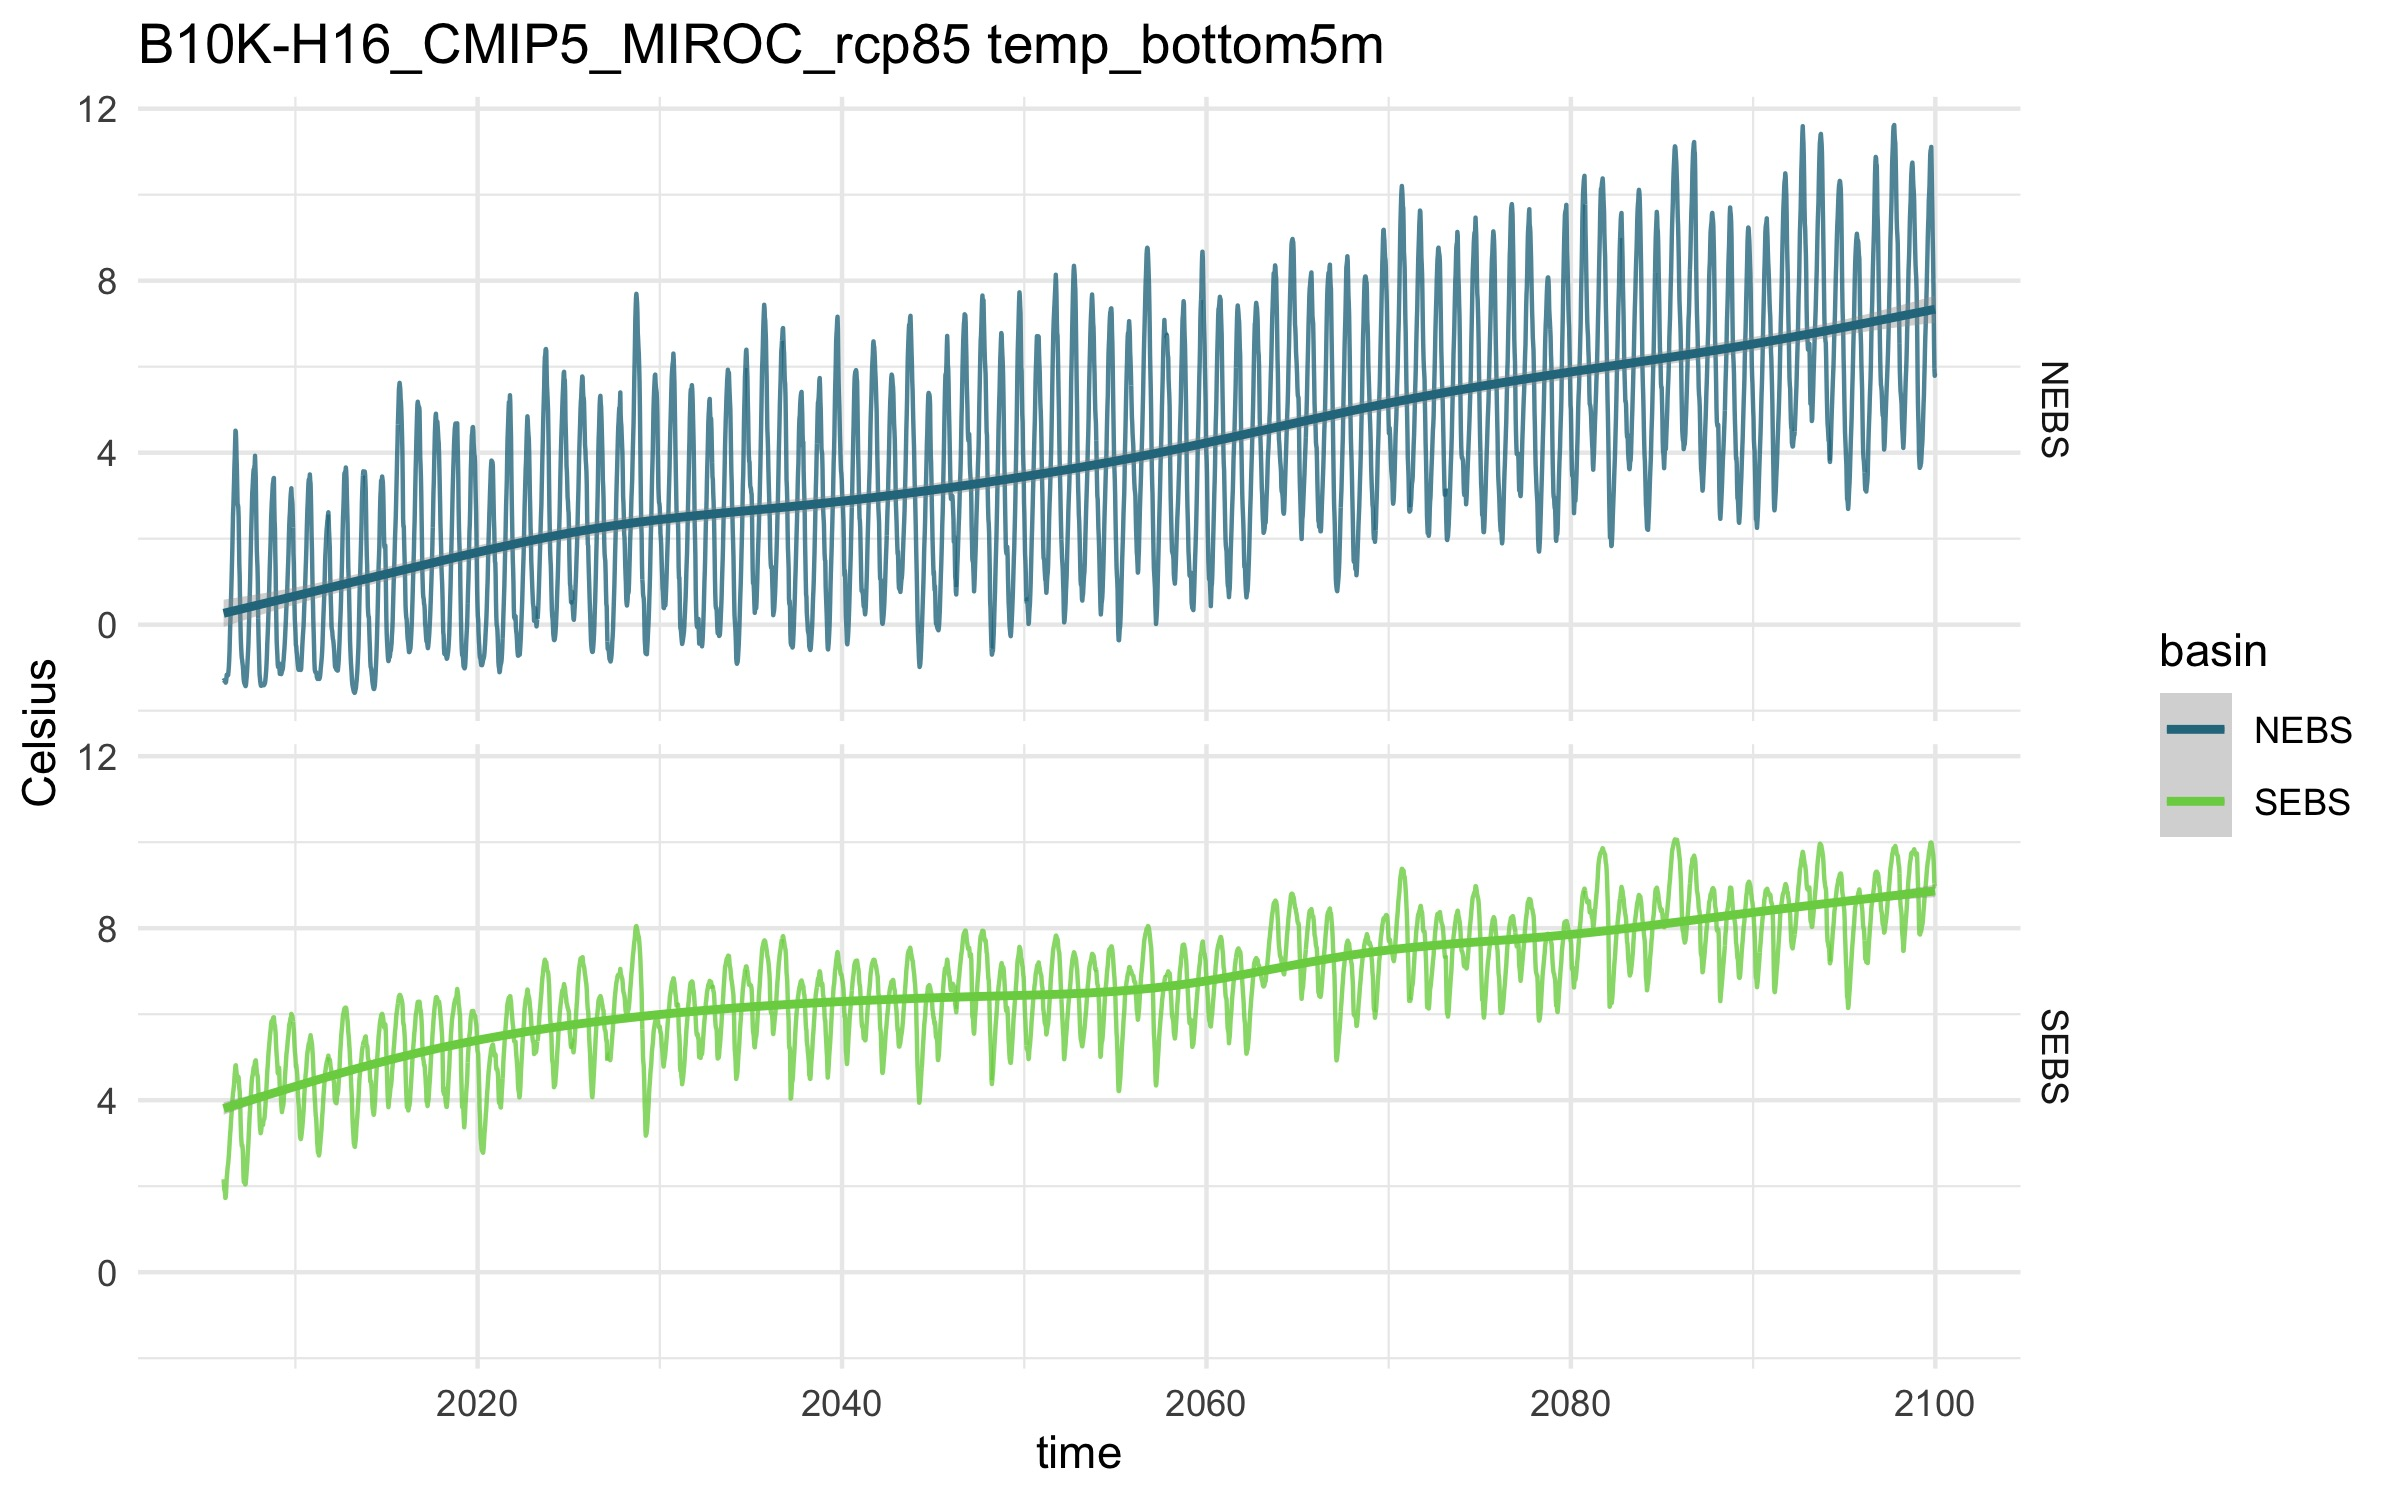
\includegraphics[width=0.65\textwidth,height=\textheight]{Figs/weekly_byreg.jpg}
\caption{Weekly indcices by sub-region}
\end{figure}

\hypertarget{create-seasonal-averages}{%
\subsubsection{4.1.4 Create seasonal
averages}\label{create-seasonal-averages}}

Now using a similar approach get the monthly mean values for a variable:

\begin{Shaded}
\begin{Highlighting}[]
\NormalTok{    sim <-}\StringTok{"B10K-K20P19_CMIP6_miroc_ssp585"} 

    \CommentTok{# Set up seasons (this follows Holsman et al. 2020)}
\NormalTok{      seasons <-}\StringTok{ }\KeywordTok{data.frame}\NormalTok{(}\DataTypeTok{mo =} \DecValTok{1}\OperatorTok{:}\DecValTok{12}\NormalTok{, }
                   \DataTypeTok{season =}\KeywordTok{factor}\NormalTok{(}\StringTok{""}\NormalTok{,}
                     \DataTypeTok{levels=}\KeywordTok{c}\NormalTok{(}\StringTok{"Winter"}\NormalTok{,}\StringTok{"Spring"}\NormalTok{,}\StringTok{"Summer"}\NormalTok{,}\StringTok{"Fall"}\NormalTok{)))}
\NormalTok{      seasons}\OperatorTok{$}\NormalTok{season[}\DecValTok{1}\OperatorTok{:}\DecValTok{3}\NormalTok{]   <-}\StringTok{ "Winter"}
\NormalTok{      seasons}\OperatorTok{$}\NormalTok{season[}\DecValTok{4}\OperatorTok{:}\DecValTok{6}\NormalTok{]   <-}\StringTok{ "Spring"}
\NormalTok{      seasons}\OperatorTok{$}\NormalTok{season[}\DecValTok{7}\OperatorTok{:}\DecValTok{9}\NormalTok{]   <-}\StringTok{ "Summer"}
\NormalTok{      seasons}\OperatorTok{$}\NormalTok{season[}\DecValTok{10}\OperatorTok{:}\DecValTok{12}\NormalTok{] <-}\StringTok{ "Fall"}
    
       
\NormalTok{    varlist <-}\StringTok{ }\KeywordTok{c}\NormalTok{(}
                  \StringTok{"temp_bottom5m"}\NormalTok{,}
                  \StringTok{"NCaS_integrated"}\NormalTok{, }\CommentTok{# Large Cop}
                  \StringTok{"Cop_integrated"}\NormalTok{,  }\CommentTok{# Small Cop}
                  \StringTok{"EupS_integrated"}\NormalTok{) }\CommentTok{# Euphausiids}
    
    \CommentTok{# open a "region" or strata specific  file}
\NormalTok{    fl      <-}\StringTok{ }\KeywordTok{file.path}\NormalTok{(sim,}\KeywordTok{paste0}\NormalTok{(reg_txt,sim,}\StringTok{".Rdata"}\NormalTok{))}
    \KeywordTok{load}\NormalTok{(}\KeywordTok{file.path}\NormalTok{(Rdata_path,fl))}
    
\NormalTok{    tmp_var1     <-}\StringTok{ }\NormalTok{ACLIMregion}\OperatorTok
\StringTok{      }\KeywordTok{filter}\NormalTok{(var}\OperatorTok\NormalTok{varlist[}\DecValTok{1}\NormalTok{])}\OperatorTok
\StringTok{      }\KeywordTok{group_by}\NormalTok{(time,strata,strata_area_km2,basin)}
    
\NormalTok{     tmp_var3     <-}\StringTok{ }\NormalTok{ACLIMregion}\OperatorTok
\StringTok{      }\KeywordTok{filter}\NormalTok{(var}\OperatorTok\NormalTok{varlist[}\DecValTok{3}\NormalTok{])}\OperatorTok
\StringTok{      }\KeywordTok{group_by}\NormalTok{(time,strata,strata_area_km2,basin)}
    
\NormalTok{    tmp_var     <-}\KeywordTok{merge}\NormalTok{(tmp_var1,tmp_var3,}
                        \DataTypeTok{by=}\KeywordTok{c}\NormalTok{(}\StringTok{"strata"}\NormalTok{,}
                             \StringTok{"strata_area_km2"}
\NormalTok{                             ,}\StringTok{"time"}\NormalTok{,}\StringTok{"basin"}\NormalTok{))}
\NormalTok{    tmp_var     <-tmp_var}\OperatorTok
\StringTok{      }\KeywordTok{mutate}\NormalTok{(}\DataTypeTok{val      =}\NormalTok{ val.x }\OperatorTok{+}\StringTok{ }\NormalTok{val.y ,}\DataTypeTok{units =}\NormalTok{ units.x,}
             \DataTypeTok{var       =} \StringTok{"Zoop_integrated"}\NormalTok{,}
             \DataTypeTok{long_name =}\StringTok{"Total On-shelf }
\StringTok{             large zooplankton concentration, }
\StringTok{             integrated over depth (NCa, Eup)"}\NormalTok{)}\OperatorTok
\StringTok{      }\KeywordTok{select}\NormalTok{(time,}
\NormalTok{             strata,}
\NormalTok{             strata_area_km2,}
\NormalTok{             basin,}
\NormalTok{             var,}
\NormalTok{             val, }
\NormalTok{             units,}
\NormalTok{             long_name)}
    \KeywordTok{rm}\NormalTok{(ACLIMregion)}
    \KeywordTok{head}\NormalTok{(tmp_var)}
    
\NormalTok{    tmp_var}\OperatorTok{$}\NormalTok{yr     <-}\StringTok{ }\KeywordTok{strptime}\NormalTok{(}\KeywordTok{as.Date}\NormalTok{(tmp_var}\OperatorTok{$}\NormalTok{time),}
                               \DataTypeTok{format=}\StringTok{"%Y-%m-%d"}\NormalTok{)}\OperatorTok{$}\NormalTok{year }\OperatorTok{+}\StringTok{ }\DecValTok{1900}
\NormalTok{    tmp_var}\OperatorTok{$}\NormalTok{mo     <-}\StringTok{ }\KeywordTok{strptime}\NormalTok{(}\KeywordTok{as.Date}\NormalTok{(tmp_var}\OperatorTok{$}\NormalTok{time),}
                               \DataTypeTok{format=}\StringTok{"%Y-%m-%d"}\NormalTok{)}\OperatorTok{$}\NormalTok{mon  }\OperatorTok{+}\StringTok{ }\DecValTok{1}
\NormalTok{    tmp_var}\OperatorTok{$}\NormalTok{jday   <-}\StringTok{ }\KeywordTok{strptime}\NormalTok{(}\KeywordTok{as.Date}\NormalTok{(tmp_var}\OperatorTok{$}\NormalTok{time),}
                               \DataTypeTok{format=}\StringTok{"%Y-%m-%d"}\NormalTok{)}\OperatorTok{$}\NormalTok{yday }\OperatorTok{+}\StringTok{ }\DecValTok{1}
\NormalTok{    tmp_var}\OperatorTok{$}\NormalTok{season <-}\StringTok{ }\NormalTok{seasons[tmp_var}\OperatorTok{$}\NormalTok{mo,}\DecValTok{2}\NormalTok{]}
    
    \CommentTok{# To get the average value for a set of strata, weight the val by the area: (slow...)}
\NormalTok{    mn_NEBS_season <-}\StringTok{ }\KeywordTok{getAVGnSUM}\NormalTok{(}
      \DataTypeTok{strataIN =}\NormalTok{ NEBS_strata,}
      \DataTypeTok{dataIN =}\NormalTok{ tmp_var,}
      \DataTypeTok{tblock=}\KeywordTok{c}\NormalTok{(}\StringTok{"yr"}\NormalTok{,}\StringTok{"season"}\NormalTok{))}
\NormalTok{    mn_NEBS_season}\OperatorTok{$}\NormalTok{basin =}\StringTok{ "NEBS"}
\NormalTok{    mn_SEBS_season <-}\StringTok{ }\KeywordTok{getAVGnSUM}\NormalTok{(}
      \DataTypeTok{strataIN =}\NormalTok{ SEBS_strata, }
      \DataTypeTok{dataIN =}\NormalTok{ tmp_var,}
      \DataTypeTok{tblock=}\KeywordTok{c}\NormalTok{(}\StringTok{"yr"}\NormalTok{,}\StringTok{"season"}\NormalTok{))}
\NormalTok{    mn_SEBS_season}\OperatorTok{$}\NormalTok{basin =}\StringTok{ "SEBS"}
    
\NormalTok{    plot_data      <-}\StringTok{ }\KeywordTok{rbind}\NormalTok{(mn_NEBS_season,mn_SEBS_season)}
    
   \CommentTok{# plot Fall values:}
\NormalTok{   p6 <-}\StringTok{ }\KeywordTok{ggplot}\NormalTok{(}\DataTypeTok{data =}\NormalTok{ plot_data}\OperatorTok\KeywordTok{filter}\NormalTok{(season}\OperatorTok{==}\StringTok{"Fall"}\NormalTok{) ) }\OperatorTok{+}\StringTok{ }
\StringTok{      }\KeywordTok{geom_line}\NormalTok{(   }\KeywordTok{aes}\NormalTok{(}\DataTypeTok{x =}\NormalTok{ yr,}\DataTypeTok{y =}\NormalTok{ mn_val,}\DataTypeTok{color=}\NormalTok{basin),}\DataTypeTok{alpha=}\NormalTok{.}\DecValTok{8}\NormalTok{)}\OperatorTok{+}
\StringTok{      }\KeywordTok{geom_smooth}\NormalTok{( }\KeywordTok{aes}\NormalTok{(}\DataTypeTok{x =}\NormalTok{ yr,}\DataTypeTok{y =}\NormalTok{ mn_val,}\DataTypeTok{color=}\NormalTok{basin),}
                  \DataTypeTok{formula =}\NormalTok{ y }\OperatorTok{~}\StringTok{ }\NormalTok{x, }\DataTypeTok{se =}\NormalTok{ T)}\OperatorTok{+}
\StringTok{      }\KeywordTok{facet_grid}\NormalTok{(basin}\OperatorTok{~}\NormalTok{.)}\OperatorTok{+}
\StringTok{      }\KeywordTok{scale_color_viridis_d}\NormalTok{(}\DataTypeTok{begin=}\NormalTok{.}\DecValTok{4}\NormalTok{,}\DataTypeTok{end=}\NormalTok{.}\DecValTok{8}\NormalTok{)}\OperatorTok{+}
\StringTok{      }\KeywordTok{ylab}\NormalTok{(tmp_var}\OperatorTok{$}\NormalTok{units[}\DecValTok{1}\NormalTok{])}\OperatorTok{+}
\StringTok{      }\KeywordTok{ggtitle}\NormalTok{( }\KeywordTok{paste}\NormalTok{(sim,}\StringTok{"Fall"}\NormalTok{,mn_NEBS_season}\OperatorTok{$}\NormalTok{var[}\DecValTok{1}\NormalTok{]))}\OperatorTok{+}
\StringTok{      }\KeywordTok{theme_minimal}\NormalTok{()}
\NormalTok{  p6}
  
  
  \ControlFlowTok{if}\NormalTok{(update.figs)  }
    \KeywordTok{ggsave}\NormalTok{(}\DataTypeTok{file=}\StringTok{"Figs/Fall_large_Zoop.jpg"}\NormalTok{,}\DataTypeTok{width=}\DecValTok{8}\NormalTok{,}\DataTypeTok{height=}\DecValTok{5}\NormalTok{)}
\end{Highlighting}
\end{Shaded}

\begin{figure}
\centering
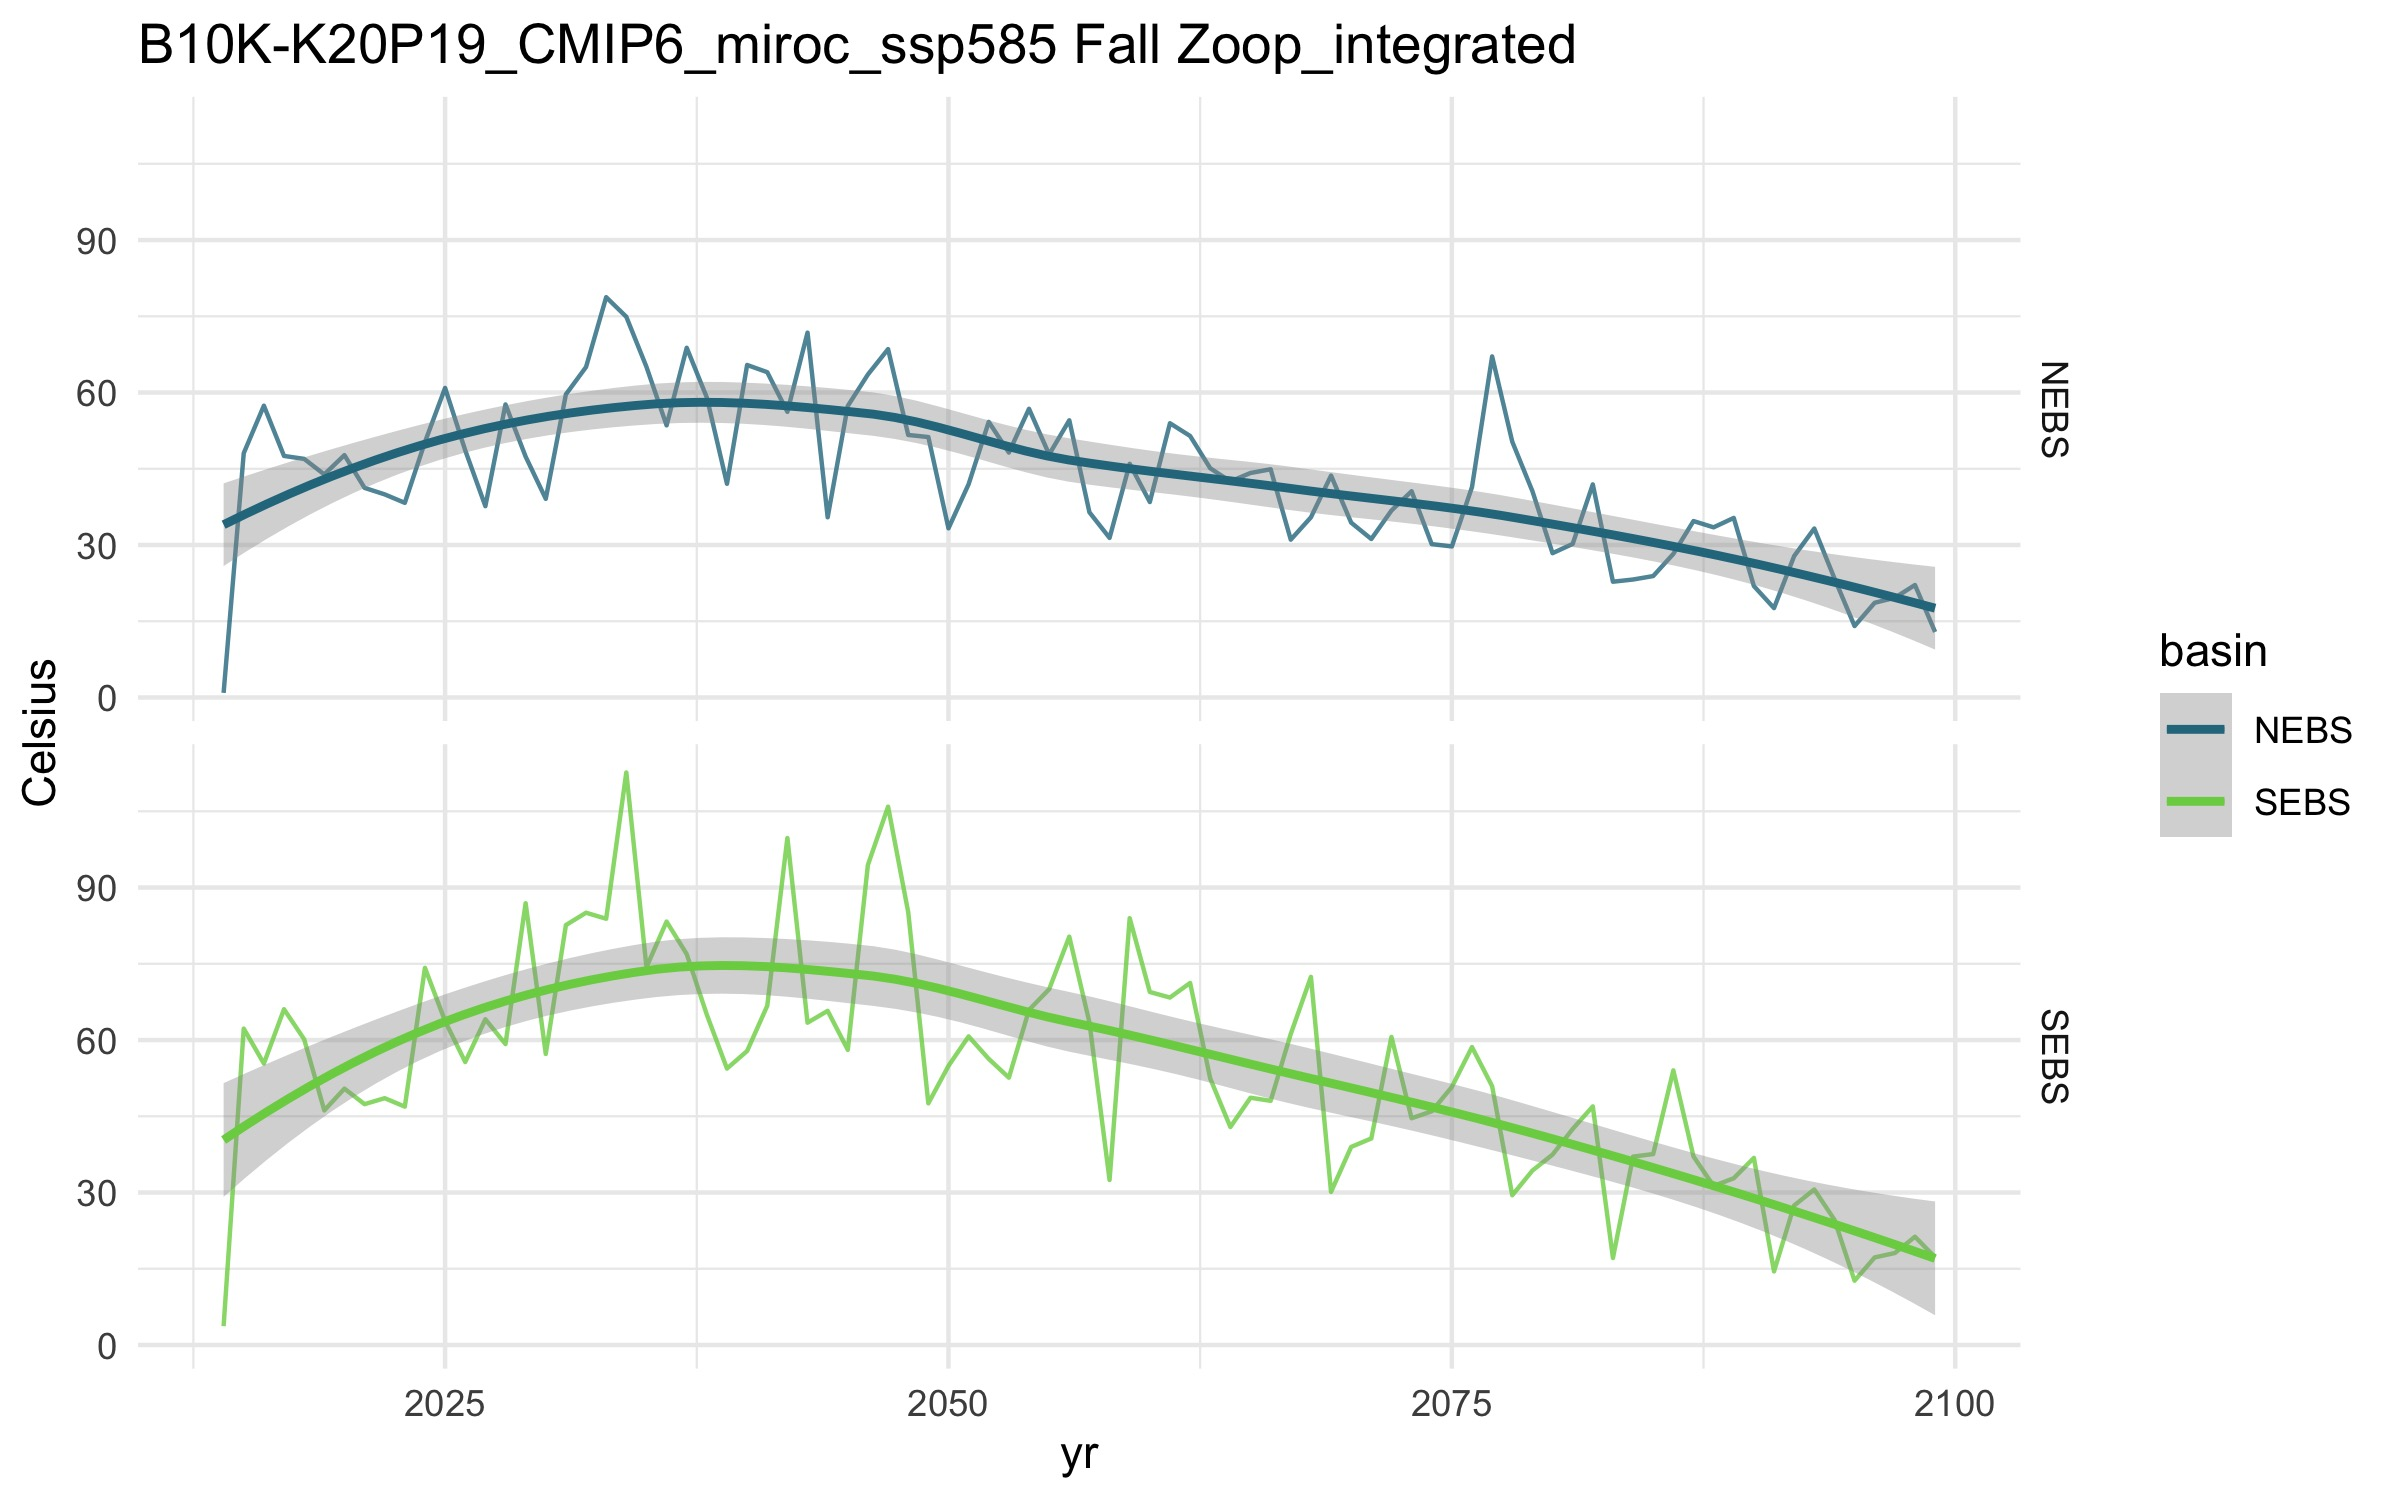
\includegraphics[width=0.65\textwidth,height=\textheight]{Figs/Fall_large_Zoop.jpg}
\caption{Large fall zooplankton integrated concentration}
\end{figure}

\hypertarget{create-monthly-averages}{%
\subsubsection{4.1.5 Create monthly
averages}\label{create-monthly-averages}}

Using the same approach we can get monthly averages for a given
variable:

\begin{Shaded}
\begin{Highlighting}[]
    \CommentTok{# To get the average value for a set of strata, weight the val by the area: (slow...)}
\NormalTok{    mn_NEBS_season <-}\StringTok{ }\KeywordTok{getAVGnSUM}\NormalTok{(}
      \DataTypeTok{strataIN =}\NormalTok{ NEBS_strata,}
      \DataTypeTok{dataIN =}\NormalTok{ tmp_var,}
      \DataTypeTok{tblock=}\KeywordTok{c}\NormalTok{(}\StringTok{"yr"}\NormalTok{,}\StringTok{"mo"}\NormalTok{))}
\NormalTok{    mn_NEBS_season}\OperatorTok{$}\NormalTok{basin =}\StringTok{ "NEBS"}
\NormalTok{    mn_SEBS_season <-}\StringTok{ }\KeywordTok{getAVGnSUM}\NormalTok{(}
      \DataTypeTok{strataIN =}\NormalTok{ SEBS_strata, }
      \DataTypeTok{dataIN =}\NormalTok{ tmp_var,}
      \DataTypeTok{tblock=}\KeywordTok{c}\NormalTok{(}\StringTok{"yr"}\NormalTok{,}\StringTok{"mo"}\NormalTok{))}
\NormalTok{    mn_SEBS_season}\OperatorTok{$}\NormalTok{basin =}\StringTok{ "SEBS"}
    
\NormalTok{    plot_data      <-}\StringTok{ }\KeywordTok{rbind}\NormalTok{(mn_NEBS_season,mn_SEBS_season)}
    
   \CommentTok{# plot Fall values:}
\NormalTok{   p7 <-}\StringTok{ }\KeywordTok{ggplot}\NormalTok{(}\DataTypeTok{data =}\NormalTok{ plot_data}\OperatorTok\KeywordTok{filter}\NormalTok{(mo}\OperatorTok{==}\DecValTok{9}\NormalTok{) ) }\OperatorTok{+}\StringTok{ }
\StringTok{      }\KeywordTok{geom_line}\NormalTok{(   }\KeywordTok{aes}\NormalTok{(}\DataTypeTok{x =}\NormalTok{ yr,}\DataTypeTok{y =}\NormalTok{ mn_val,}\DataTypeTok{color=}\NormalTok{basin),}\DataTypeTok{alpha=}\NormalTok{.}\DecValTok{8}\NormalTok{)}\OperatorTok{+}
\StringTok{      }\KeywordTok{geom_smooth}\NormalTok{( }\KeywordTok{aes}\NormalTok{(}\DataTypeTok{x =}\NormalTok{ yr,}\DataTypeTok{y =}\NormalTok{ mn_val,}\DataTypeTok{color=}\NormalTok{basin),}
                  \DataTypeTok{formula =}\NormalTok{ y }\OperatorTok{~}\StringTok{ }\NormalTok{x, }\DataTypeTok{se =}\NormalTok{ T)}\OperatorTok{+}
\StringTok{      }\KeywordTok{facet_grid}\NormalTok{(basin}\OperatorTok{~}\NormalTok{.)}\OperatorTok{+}
\StringTok{      }\KeywordTok{scale_color_viridis_d}\NormalTok{(}\DataTypeTok{begin=}\NormalTok{.}\DecValTok{4}\NormalTok{,}\DataTypeTok{end=}\NormalTok{.}\DecValTok{8}\NormalTok{)}\OperatorTok{+}
\StringTok{      }\KeywordTok{ylab}\NormalTok{(tmp_var}\OperatorTok{$}\NormalTok{units[}\DecValTok{1}\NormalTok{])}\OperatorTok{+}
\StringTok{      }\KeywordTok{ggtitle}\NormalTok{( }\KeywordTok{paste}\NormalTok{(aclim[}\DecValTok{2}\NormalTok{],}\StringTok{"Sept."}\NormalTok{,mn_NEBS_season}\OperatorTok{$}\NormalTok{var[}\DecValTok{1}\NormalTok{]))}\OperatorTok{+}
\StringTok{      }\KeywordTok{theme_minimal}\NormalTok{()}
\NormalTok{  p7}
  
  \ControlFlowTok{if}\NormalTok{(update.figs)  }
    \KeywordTok{ggsave}\NormalTok{(}\DataTypeTok{file=}\StringTok{"Figs/Sept_large_Zoop.jpg"}\NormalTok{,}\DataTypeTok{width=}\DecValTok{8}\NormalTok{,}\DataTypeTok{height=}\DecValTok{5}\NormalTok{)}
\end{Highlighting}
\end{Shaded}

\begin{figure}
\centering
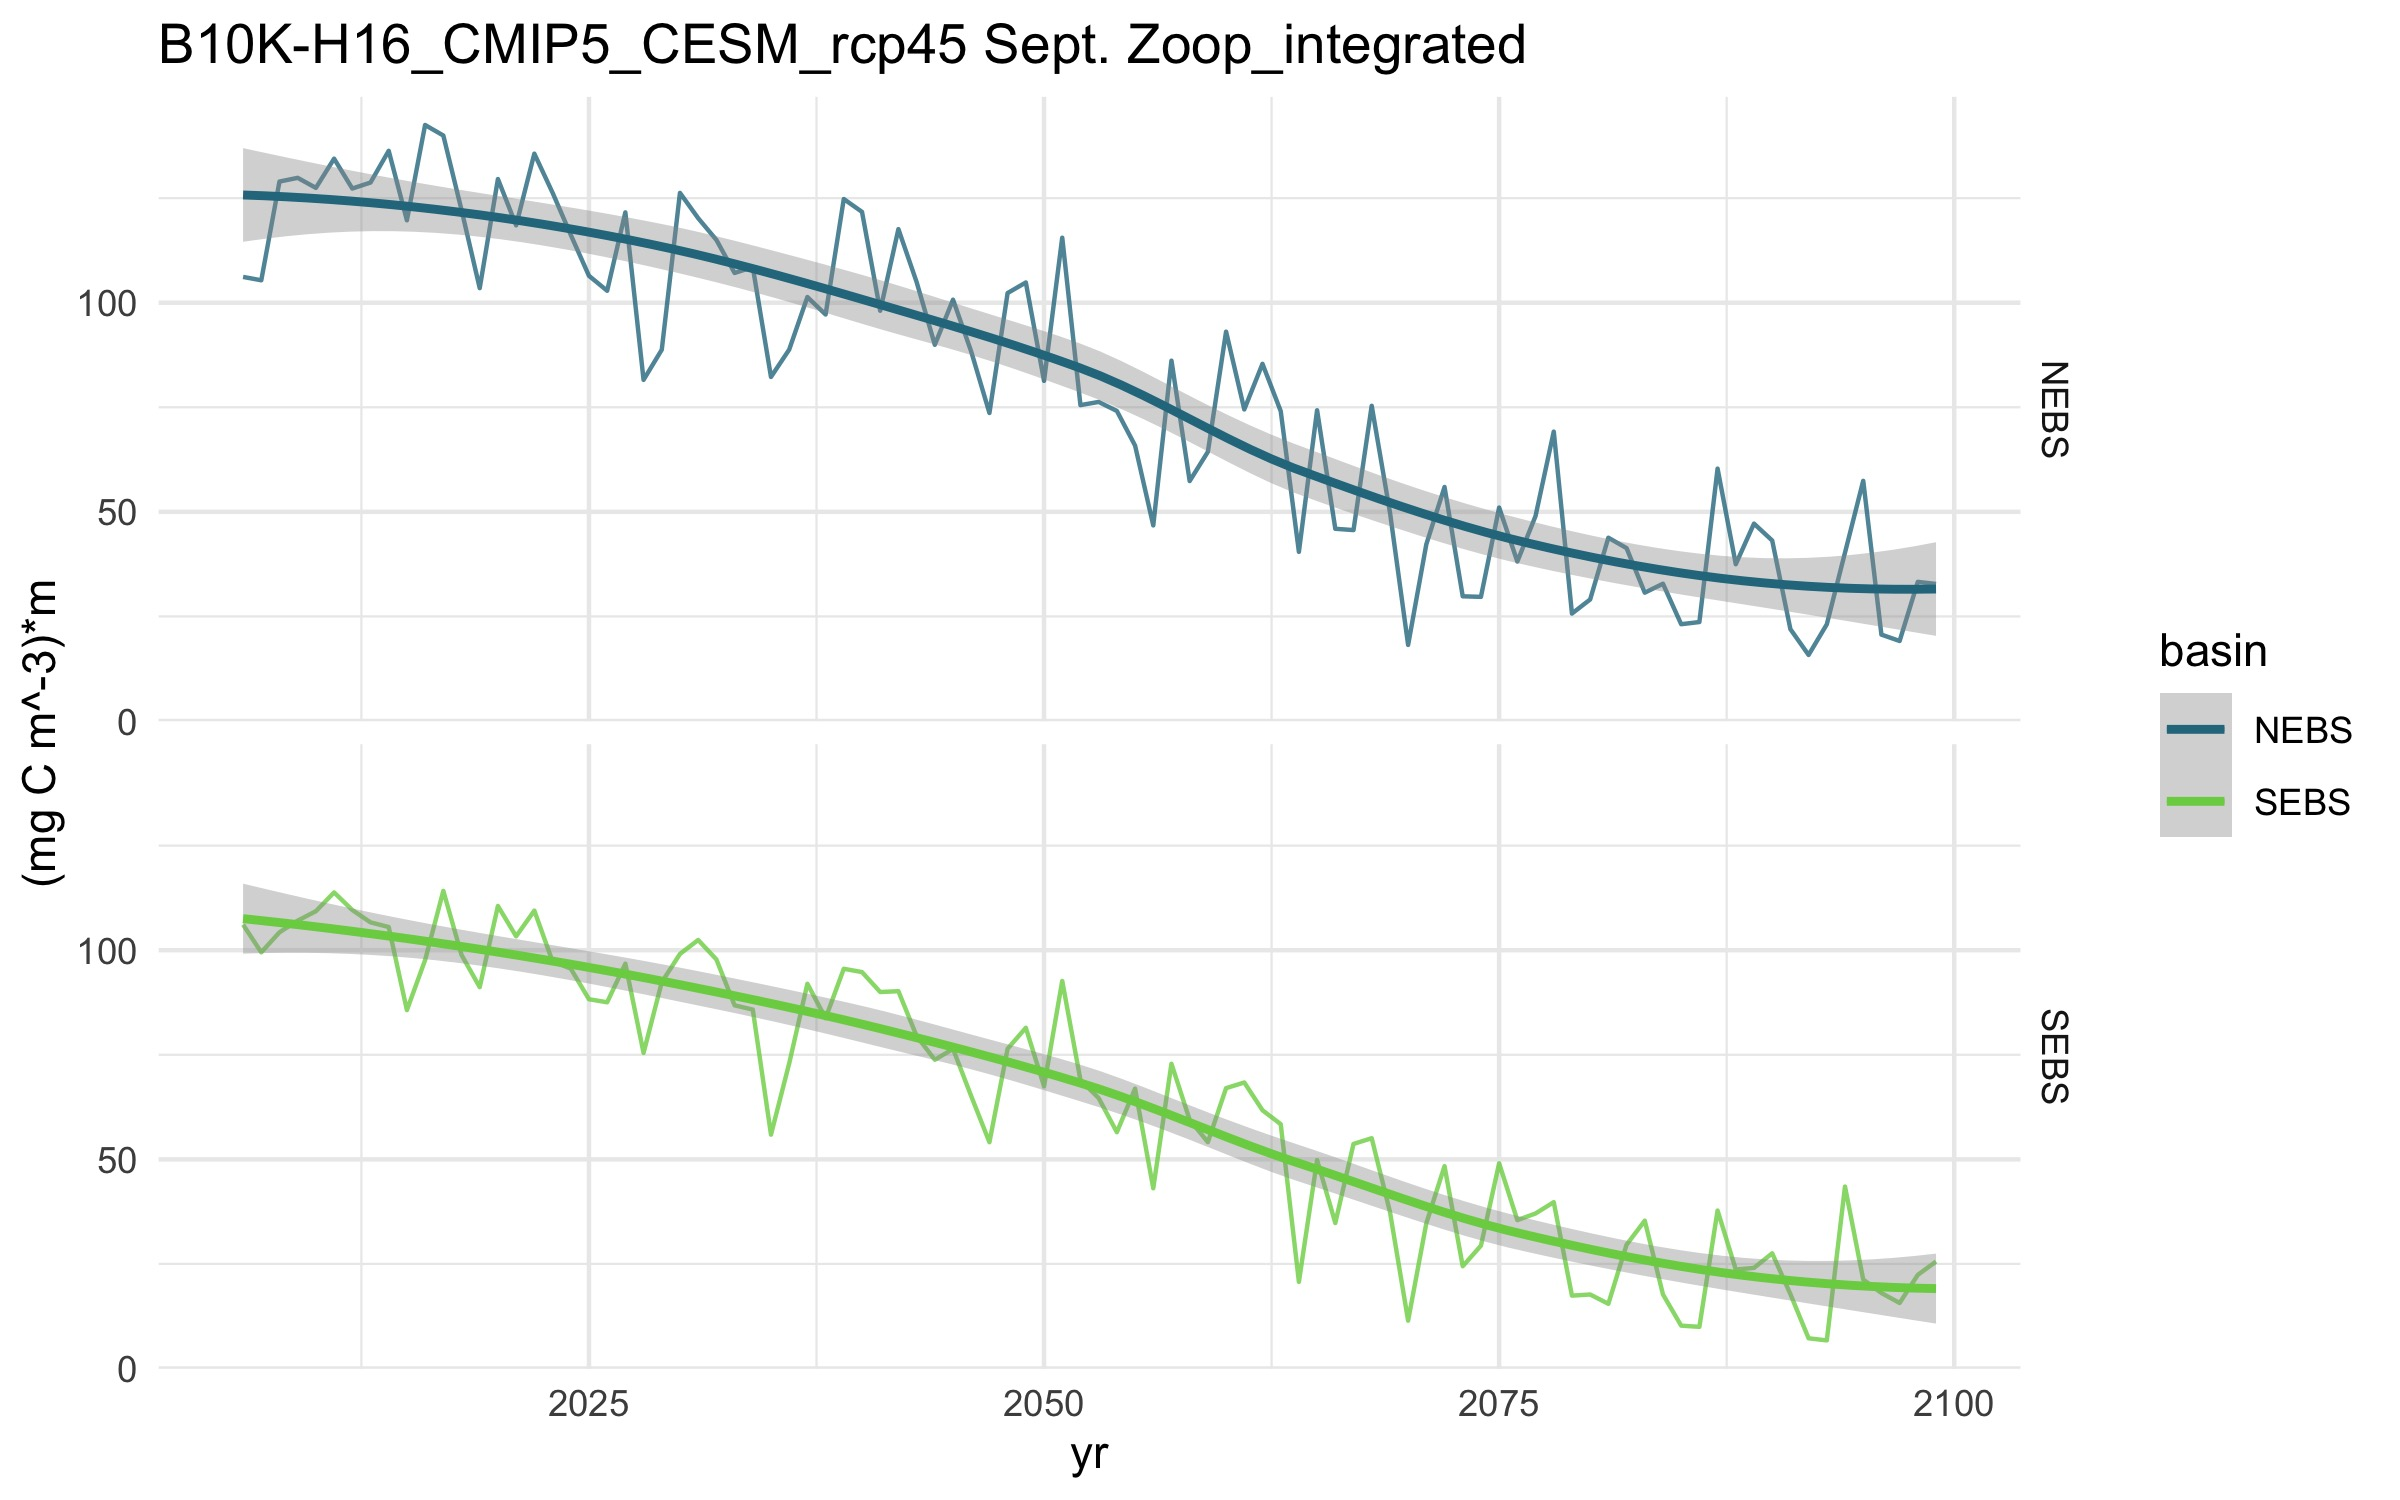
\includegraphics[width=0.65\textwidth,height=\textheight]{Figs/Sept_large_Zoop.jpg}
\caption{September large zooplankton integrated concentration}
\end{figure}

\hypertarget{level-2}{%
\subsection{4.2 Level 2:}\label{level-2}}

\hypertarget{explore-level-2-data-catalog}{%
\subsubsection{3.2.1 Explore Level 2 data
catalog}\label{explore-level-2-data-catalog}}

\hypertarget{custom-temporal-indices}{%
\subsubsection{3.2.2 Custom temporal
indices}\label{custom-temporal-indices}}

\hypertarget{custom-spatial-indices}{%
\subsubsection{3.2.3 Custom spatial
indices}\label{custom-spatial-indices}}

\hypertarget{tinker-example-applications}{%
\section{5. Tinker: example
applications}\label{tinker-example-applications}}

\hypertarget{recruitment-faclim-indices}{%
\section{5.1 Recruitment \textasciitilde f(ACLIM
indices)}\label{recruitment-faclim-indices}}

\hypertarget{spatial-overlap-fspp-dist-aclim-indices}{%
\section{5.2 Spatial overlap \textasciitilde f(spp dist, aclim
indices)}\label{spatial-overlap-fspp-dist-aclim-indices}}

\hypertarget{funding-and-acknowledgments-needs-updating}{%
\section{6. Funding and acknowledgments (needs
updating):}\label{funding-and-acknowledgments-needs-updating}}

\hypertarget{please-include-a-statement-like-the-following-one-in-your-acknowledgements-section}{%
\subsubsection{PLEASE Include a statement like the following one in your
acknowledgements
section:}\label{please-include-a-statement-like-the-following-one-in-your-acknowledgements-section}}

\emph{This study is part of NOAA's Alaska Climate Integrated Modeling
project (ACLIM) and FATE project XXXX. We would like to that the entire
ACLIM team including \texttt{{[}add\ specific\ names{]}} for feedback
and discussions on the broader application of this work. Multiple NOAA
National Marine Fisheries programs provided support for ACLIM including
Fisheries and the Environment (FATE), Stock Assessment Analytical
Methods (SAAM) Science and Technology North Pacific Climate Regimes and
Ecosystem Productivity, the Integrated Ecosystem Assessment Program
(IEA), the NOAA Economics and Social Analysis Division, NOAA Research
Transition Acceleration Program (RTAP), the Alaska Fisheries Science
Center (ASFC), the Office of Oceanic and Atmospheric Research (OAR) and
the National Marine Fisheries Service (NMFS). The scientific views,
opinions, and conclusions expressed herein are solely those of the
authors and do not represent the views, opinions, or conclusions of NOAA
or the Department of Commerce.}

\hypertarget{for-some-of-the-integrated-papers-the-following-maybe-should-also-be-added}{%
\subsubsection{For some of the integrated papers the following maybe
should also be
added:}\label{for-some-of-the-integrated-papers-the-following-maybe-should-also-be-added}}

\emph{Additionally, the International Council for the Exploration of the
Sea (ICES) and the North Pacific Marine Science Organization (PICES)
provided support for Strategic Initiative for the Study of Climate
Impacts on Marine Ecosystems (SI-CCME) workshops, which facilitated
development of the ideas presented in this paper. The scientific views,
opinions, and conclusions expressed herein are solely those of the
authors and do not represent the views, opinions, or conclusions of
NOAA, the Department of Commerce, ICES, or PICES.}

\hypertarget{helpful-links-and-further-reading}{%
\section{7. Helpful links and further
reading:}\label{helpful-links-and-further-reading}}

\hypertarget{citations-for-gcms-and-carbon-scenarios}{%
\subsection{7.1 Citations for GCMs and carbon
scenarios:}\label{citations-for-gcms-and-carbon-scenarios}}

\hypertarget{cmip3-bsierp-global-climate-model-runs}{%
\subsubsection{CMIP3 (BSIERP global climate model
runs):}\label{cmip3-bsierp-global-climate-model-runs}}

Meehl, G. A., C. Covey, T. Delworth, M. Latif, B. McAvaney, J. F. B.
Mitchell, R. J. Stouffer, and K. E. Taylor, 2007: The WCRP CMIP3
multimodel dataset: A new era in climate change research. Bull. Amer.
Meteor. Soc., 88, 1383--1394.

\hypertarget{cmip5-aclim-global-climate-model-runs}{%
\subsubsection{CMIP5 (ACLIM global climate model
runs):}\label{cmip5-aclim-global-climate-model-runs}}

Taylor, K. E., R. J. Stouffer, and G. A. Meehl, 2012:Anoverview of CMIP5
and the experiment design. Bull. Amer. Meteor. Soc., 93, 485--498.

\hypertarget{cmip6-and-ssps-aclim2-global-climate-model-runs}{%
\subsubsection{CMIP6 and SSPs (ACLIM2 global climate model
runs):}\label{cmip6-and-ssps-aclim2-global-climate-model-runs}}

ONeill, B. C., C. Tebaldi, D. P. van Vuuren, V. Eyring, P.
Friedlingstein, G. Hurtt, R. Knutti, E. Kriegler, J.-F. Lamarque, J.
Lowe, G. A. Meehl, R. Moss, K. Riahi, and B. M. Sanderson. 2016. The
Scenario Model Intercomparison Project (ScenarioMIP) for CMIP6.
Geoscientific Model Development 9:3461--3482.

\hypertarget{weblinks-for-further-reading}{%
\subsection{7.2 Weblinks for further
reading:}\label{weblinks-for-further-reading}}

\begin{itemize}
\item
  Explore annual indices of downscaled projections for the EBS:
  \href{https://kholsman.shinyapps.io/aclim/}{\textbf{ACLIM indices}}
\item
  To view climate change projections from CMIP5 (eventually
  CMIP6):\href{https://www.esrl.noaa.gov/psd/ipcc/ocn/}{\textbf{ESRL
  climate change portal }}
\end{itemize}

\hypertarget{additional-information-on-hindcast-and-projection-models-needs-updating}{%
\subsection{7.3 Additional information on Hindcast and Projection Models
(needs
updating)}\label{additional-information-on-hindcast-and-projection-models-needs-updating}}

\hypertarget{core-cfsr-1976-2012}{%
\subsubsection{CORE-CFSR (1976-2012)}\label{core-cfsr-1976-2012}}

This is the hindcast for the Bering Sea and is a combination of the
reconstructed climatology from the
\href{http://portal.aoos.org/bering-sea.php\#module-metadata/5626a0b6-7d79-11e3-ac17-00219bfe5678/0756e6c2-a8e2-40af-aa3d-22051ed68067}{\textbf{CLIVAR}}
Co-ordinated Ocean-Ice Reference Experiments (CORE) Climate Model
(1969-2006) the
\href{http://portal.aoos.org/bering-sea.php\#module-metadata/f8cb79f6-7d59-11e3-a6ee-00219bfe5678/2deb2eca-f3f5-4eda-a132-112468711de7}{\textbf{NCEP}}
Climate Forecast System Reanalysis is a set of re-forecasts carried out
by NOAA's National Center for Environmental Prediction (NCEP). See
\href{http://cfs.ncep.noaa.gov/cfsr/}{\textbf{CFS-R}} for more info.

\hypertarget{cccma2006-2039-ar4-sres-a1b}{%
\subsubsection{\texorpdfstring{\href{http://www.cccma.ec.gc.ca/diagnostics/cgcm3/cgcm3.shtml}{CCCMA}(2006-2039;
AR4 SRES
A1B)}{CCCMA(2006-2039; AR4 SRES A1B)}}\label{cccma2006-2039-ar4-sres-a1b}}

Developed by the Canadian Centre for Climate Modelling and Analysis,
this is also known as the CGCM3/T47 model. This model showed the
greatest warming over time compared to other models tested by PMEL. See
more data the
\href{http://portal.aoos.org/bering-sea.php\#module-metadata/4f706756-7d57-11e3-bce5-00219bfe5678/ffa1bcc1-288d-4f8e-912e-500a618b241a}{\textbf{AOOS:CCCMA
portal}}.

\hypertarget{echog2006-2039-ar4-sres-a1b}{%
\subsubsection{\texorpdfstring{\href{http://www-pcmdi.llnl.gov/ipcc/model_documentation/ECHO-G.pdf}{ECHOG}(2006-2039;
AR4 SRES
A1B)}{ECHOG(2006-2039; AR4 SRES A1B)}}\label{echog2006-2039-ar4-sres-a1b}}

The ECHO-G model from the Max Planck Institute in Germany This model
showed the least warming over time compared to other models tested by
PMEL. See more data the AOOS:ECHO-G portal.

\hypertarget{gfdl-2006-2100-ar5-rcp-4.5-8.5-ssp126ssp585}{%
\subsubsection{\texorpdfstring{\href{http://www.gfdl.noaa.gov/earth-system-model}{GFDL}
(2006-2100; AR5 RCP 4.5, 8.5,
SSP126,SSP585)}{GFDL (2006-2100; AR5 RCP 4.5, 8.5, SSP126,SSP585)}}\label{gfdl-2006-2100-ar5-rcp-4.5-8.5-ssp126ssp585}}

The NOAA Geophysical Fluid Dynamics Laboratory
\href{http://www.gfdl.noaa.gov}{\textbf{GFDL}} has lead development of
the first Earth System Models (ESMs), which like physical climate
models, are based on an atmospheric circulation model coupled with an
oceanic circulation model, with representations of land, sea ice and
iceberg dynamics; ESMs additionally incorporate interactive
biogeochemistry, including the carbon cycle. The ESM2M model used in
this project is an evolution of the prototype EMS2.1 model, where
pressure-based vertical coordinates are used along the developmental
path of GFDL's Modular Ocean Model version 4.1 and where the land model
is more adavanced (LM3) than in the previous ESM2.1

\hypertarget{miroc2006-2039-ar4-sres-a1b-2006-2100-rcp4.5-rcp8.5-ssp585-ssp126}{%
\subsubsection{\texorpdfstring{\href{www.cger.nies.go.jp/publications/report/i073/I073.pdf}{MIROC}(2006-2039;
AR4 SRES A1B; 2006-2100 RCP4.5, RCP8.5, SSP585,
SSP126)}{MIROC(2006-2039; AR4 SRES A1B; 2006-2100 RCP4.5, RCP8.5, SSP585, SSP126)}}\label{miroc2006-2039-ar4-sres-a1b-2006-2100-rcp4.5-rcp8.5-ssp585-ssp126}}

The Model for Interdisciplinary Research on Climate (MIROC)-M model
developed by a consortium of agencies in Japan {[}{]}. Compared to other
models tested by PMEL, MIROC-M was intermediate in degree of warming
over the Bering Sea shelf for the first half of the 21st century. See
more data the AOOS:MIROC portal.

\end{document}
